\documentclass[12pt, a4paper]{article}
\usepackage{amsfonts, amsmath, amsthm}
\usepackage[utf8x]{inputenc}
\usepackage{indentfirst}
\usepackage{multirow}
\usepackage[table]{xcolor}
\usepackage{listings}
\usepackage{alltt}
\usepackage{fancyvrb}
\usepackage{amsmath}
\usepackage{graphicx}
\usepackage{algorithm}
\usepackage{algpseudocode}
\usepackage{subfigure}
\usepackage{setspace}
\usepackage{wrapfig}
\usepackage{colortbl}
\usepackage{wrapfig}
\usepackage{tikz}
\usepackage{subfig}
\usepackage[hyphens]{url}
\usepackage{setspace}


\usetikzlibrary{positioning}
\graphicspath{ {./images/} }


\title{%
	
\includegraphics[height=0.3\textwidth]{UNITBV2.png}~ 
	\\[1cm]
	\vspace{20mm}
	
	\bf 	LUCRARE DE LICENȚĂ
	\noindent\rule{14cm}{1pt}
	\bf Serenity Garden TD
}

\date{}

\begin{document}
	
	
	
	\maketitle
	\vspace{10mm} %5mm vertical space
	\begin{flushleft}
		\bf 	Conducător Stiintific:
		\bf     \\Lector Universitar Deaconu Adrian
	\end{flushleft}
	
	\begin{flushright}
		\bf Absolvent:
		\bf \\Opria Ion-Bogdan
	\end{flushright}
	
	\vspace{6mm} %5mm vertical space
	
	\begin{center}
		\bf Brașov, 2021 
	\end{center}
	
	
	\tableofcontents
	\pagebreak
	
	\section{Introducere}
	
	
	
	
	
	\subsection{Descrierea proiectului}
	
	Jocurile video au inceput sa acapareze din ce in ce mai mult vietile noastre datorita usurintei de accesare si a experientei pe care o ofera. Odata cu evolutia hardware-ului, jocurile video au devenit din ce in ce mai realiste si prin urmare ofera experiente care nu poat fi gasite in niciun alt mediu existent, deoarece in nici un alt mediu nu putem controla si traii experientele unor personaje atat de indetaliat. Industria jocurilor video este o industrie care este in continua crestere si prin urmare este o ramura care merita explorata din perspectiva unui programator si nu nu mai. 
	\newline
	
	"Games are great to work on because they are as much about art as they are science." \cite{gameProgrammingComplete}
	\newline
	
	Din aceste motive, am ales drept proiect pentru licenta sa fac un joc video. Jocul se numeste "Serenity Garden" si este un tower defense 3D. Experienta jocului are loc in cateva nivele special definite, in care utilizatorul trebuie sa isi protejeze baza de operatii. Exista multe tipuri diferite de inamici care vor sa distruga baza jucatorului, iar acesta, pentru a o proteja, trebuie sa construiasca un sistem defensiv. Jucatorul poate sa construiasca turnuri defensive care au diferite efecte asupra inamicilor. Inamicii ataca sistemul defensiv, sau in cazul in care lipseste, ataca direct baza jucatorului. Daca reusesc sa distruga baza, jucatorului, acesta pierde nivelul curent.
	\newline
	
	Jucatorul nu poate sa construiasca turnuri oriunde, ci are locuri predefinite unde poate sa le construiasca, locuri specificate de hexagoane colorate pe harta de joc. Odata plasat un turn, aceasta nu poate fi mutat, dar jucatorul are si un caracter invulnerabil pe care il poate muta oriunde doreste pe harta. Acest caracter va ataca inamicii automat cand nu se afla in miscare, si poate intra in turnuri pentru a le creste puterea/eficienta.
	\newline
	
	Modul care va diferentia acest joc de celelalte jocuri pe acest stil este modul de co-op. Doi jucatori se vor putea conecta prin retea si vor juca un nivel dificil care necesita cooperare si o planificare buna intre ei.
	
	
	
	
	
	\subsection{Introducere in dezvoltarea jocurilor video}
	
	
	
	
	
	
	\subsubsection{Scurta istorie}
	
	
	
	
	
	
	\subsubsection{Industria curenta}
	
	
	
	
	
	\section{Introducere in Unity}
	
	
	
	
	
	\subsection{Prezentare generala}
	
	
	
	
	
	\subsubsection{GameObject si Mesh}
	
	
	
	
	
	\subsubsection{Collider}
	
	
	
	
	
	\subsubsection{Transform si Rigidbody}
	
	
	
	
	\subsubsection{Prefab}
	
	
	
	
	
	\subsubsection{Raycast si sistemul de fizica}
	
	
	
	
	
	\subsection{Motivul alegerii pentru proiectul de licenta}





	\subsection{Elemente specifice folosite}	
	
	
	
	
	
	\subsubsection{Editoare personalizate}
	
	
	
	
	
	\subsubsection{Shader Graph}
	
	
	
	
	
	\subsubsection{VFX Graph}
	
	
	
	
	
	\subsubsection{Photon Engine}
	
	
	
	
	
	\section{Planificare Proiect}
	
	
	
	
	
	\subsection{Faza de Proiectare}
	
	"Almost anything that you can be good at can become a useful
	skill for a game designer." \cite{bookOfLenses}
	\newline
	
	Din proiecte precedente am realizat ca o planificare buna a unui proiect inca de la inceput poate imbunatatii calitatea proiectului explonential, asigura usurinta de adaugare a unor elemente noi (fara sa fie necesara rescrierea/reorganizarea proiectului) si reduce frustrarea programatorilor care lucreaza la proiect.
	\newline
	
	Din acest motiv, inca de la inceputul proiectului am incercat sa imi planific cat mai indetaliat continutul acestuia si modul in care il voi implementa.
	\newline
	
	In prima faza, mi-am scris un document de proiectare care continea descrierea si elementele jocului, privite din multe perspective.
	\newline
	
	Introducerea proiectului a fost realizata la inceputul acestui document si nu va fi reluata aici.
	
	
	
	
	
	\subsection{Tematica Jocului}
	\label{section: gamePlot}
	
	Jocul are loc in viitorul departat. Planeta ta este supra-populata, iar nivelul de poluare a ajuns la un nivel critic. Umanitatea a trecut de mult de punctul in care mai pot salva aceasta planeta. Intreaga planeta va deceda in cateva decenii, iar oamenii daca nu isi gasesc o alta locuinta intre timp, vor muri si ei impreuna cu ea. In acest scop, o armata speciala a fost formata, care are ca scop explorarea altor planete si gasirea uneia care poate suporta rasa umana.
	\newline
	
	Universul este totusi foarte periculos. Unele planete au viata extraterestra foarte agresiva, iar altele au fost distruse de experimente cibernetice esuate. Jucatorul este comandantul suprem al acestei armate care are ca scop protejarea oamenilor de stiinta care vor analiza aceste planete.
	\newline
	
	Prima faza a proiectului va contine o singura planeta care poate fi populata dar care contine multi inamici periculosi.
	\newline
	
	Planeta mama trimite resurse din cand in cand, dar numai un numar limitat de resurse pot fi trimise deodata, iar acestea dureaza mult timp sa ajunga, asa ca nu putem depinde de ele in timpul unei lupte.
	
	
	
	
	
	\subsection{Caracterele Jocului}
	
	\textbf{Comandantul} este protagonistul jocului. El este caracterul a carei perspective o vom traii pe tot parcursul jocului. In trecut a fost cobai pentru un experiment menit sa creeze super-soldati, iar in urma acestui experiment a primit o putere speciala. Poate sa isi ascunda complet prezenta fata de alti oameni sau alte creaturi. Din acest motiv, el este caracterul invulnerabil pe care il putem misca pe harta in timpul luptei.
	
	
	
	
	
	\subsubsection{Inamicii}
	\begin{itemize}
		\item \textbf{Inamicul de lupta apropiata} este un tip de inamic care poate ataca turnurile doar cand sta fix in fata lor. Are viata mai multa decat inamicii de lupta de la distanta.
		\item \textbf{Inamicul de lupta de la distanta} este un tip de inamic care poate ataca turnurile de la distanta. Are viata putina, dar pot ataca repede.
		\item \textbf{Inamicul zburator} este un inamic care poate fi lovit doar de un numar limitat de turnuri.
		\item \textbf{Inamicul bombardier} este un tip de inamic care ignora turnurile intalnite in cale. Acesta se misca pe cel mai scurt drum catre baza jucatorului, iar daca ajunge deasupra acesteia, va lansa bombe care ii vor scadea drastic viata, dupa care vor pleca de pe mapa. Este un tip de inamic zburator care poate fi lovit doar de un numar limitat de turnuri.
	\end{itemize}

	Acesti inamici (cu exceptia bombardierului) se vor misca pe harta calculand cel mai scurt drum catre baza jucatorului. Daca acestia intalnesc in cale un turn, se vor opri si vor ataca acel turn. Cand turnul este distrus, acestia isi vor relua drumul.
	\newline
	
	Pentru fiecare inamic vor fi 3 tipuri de variatii, fiecare mai puternic decat cel precedent.
	
	
	
	
	
	\subsubsection{Turnuri defensive}
	In continuare voi scrie o descriere scurta pentru fiecare turn din joc. Toate proprietatile despre care urmeaza sa vorbesc sunt in comparatie cu celelalte turnuri defensive.
	\begin{itemize}
		\item \textbf{Serenity} este baza jucatorului. Are viata foarte multa daca este distrusa jucatorul pierde nivelul curent. Aceasta poate ataca inamicii care se apropie de ea. Are raza de atac medie, putere de atac mediu, poate ataca orice tip de inamic, iar rata de reincarcare intre atacuri este mica (dureaza mult timp intre atacuri)
		\item \textbf{Mitraliera automata} (fig: \ref{fig: machineGun}) Are viata mica, poate ataca orice tip de inamic, are raza medie, putere de atac mica si rata de atac este mare (ataca foarte des)
		\item \textbf{Gardul electric} (fig: \ref{fig: electricFence}) este turnul de protectie. Are viata foarte mare, poate ataca doar inamicii de lupta apropiata, puterea de atac este medie, iar rata de reincarcare este mica. Scopul acestui turn este sa stea in calea inamicilor pentru a fi atacat de acestia, permitand celorlalte turnuri sa atace inamicii blocati.
		\item \textbf{Vulkan} (fig: \ref{fig: vulkan}) Este turnul special construit pentru a lupta impotriva inamicilor zburatori. Are viata putina, raza de atac mare si putere de atac mare dar poate ataca doar inamicii zburatori.
		\item \textbf{Aruncatorul de flacari} (fig: \ref{fig: machineCannon}). Cand inamicii intra in raza acestui turn, el va imprastia flacari catre inamici. Toti inamicii care intra in aceste flacari primesc damage in fiecare clipa in care stau in flacari. Are viata medie, ataca instant si puterea de atac este mica dar distribuita in fiecare clipa in care inamicii stau in flacarile acestui turn.
		\item \textbf{Laser} (fig: \ref{fig: railgun}). Este un turn similar cu aruncatorul de flacari in sensul in care ataca in fiecare clipa in care un inamic este in raza acestuia. Ataca cu un laser puternic care scade treptat viata inamicilor. Are viata medie, ataca instant si puterea de atac este mica.
		\item \textbf{Excavator} (fig: \ref{fig: excavator}) este un tip special de turn deoarece nu poate ataca inamicii. Acesta aduna resurse in timpul luptei, resurse care pot fi convertite in bani de joc. Are viata multa, si pentru ca nu poate ataca, trebuie sa fie aparat de inamici.
	\end{itemize}
	
	
	%\begin{figure}[H]
	%	\centering
	%	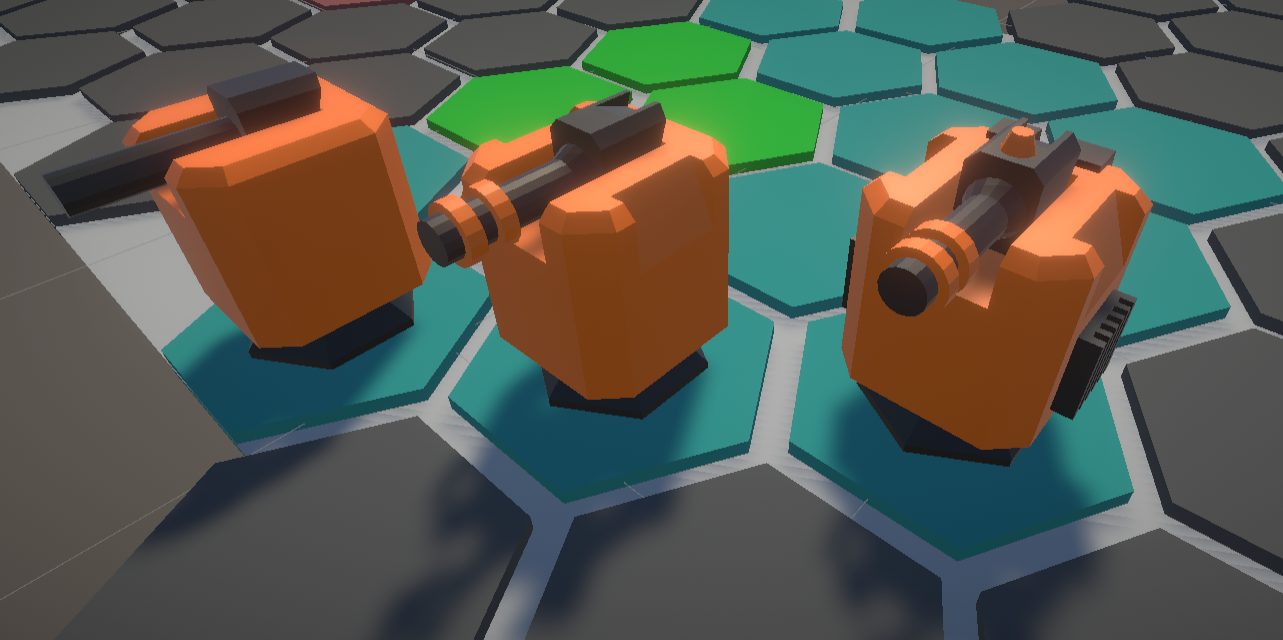
\includegraphics[width=1\textwidth]{machineGun.png}
	%	\caption{Mitraliera automata}
	%	\label{fig: machineGun}
	%\end{figure}

	%\begin{figure}[H]
	%	\centering
	%	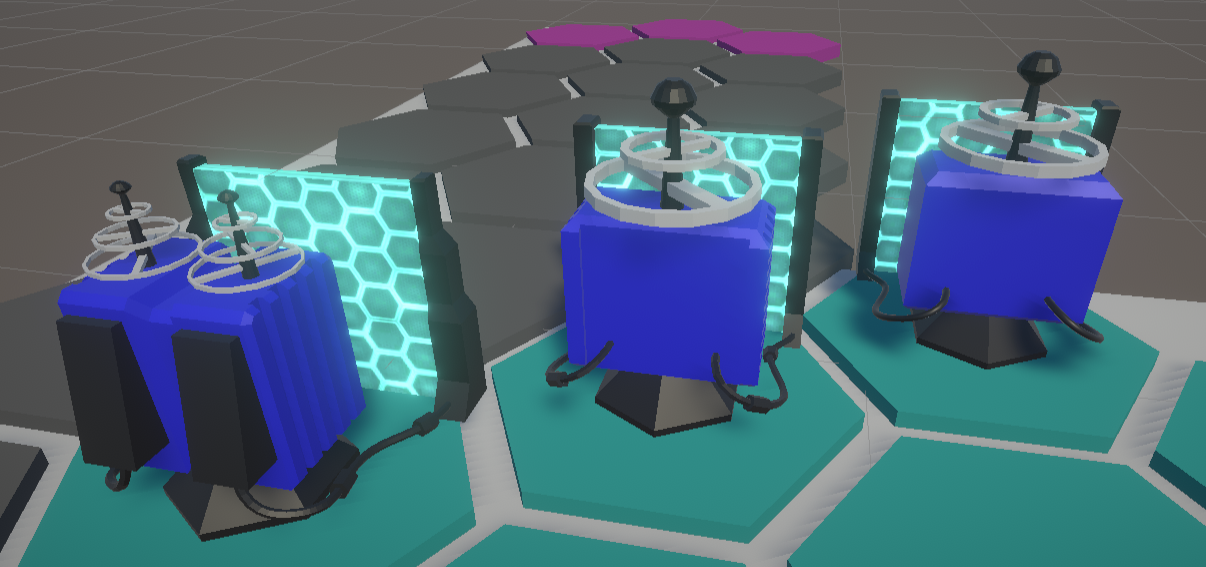
\includegraphics[width=1\textwidth]{electricFence.png}
	%	\caption{Gardul electric}
	%	\label{fig: electricFence}
	%\end{figure}

	%\begin{figure}[H]
	%	\centering
	%	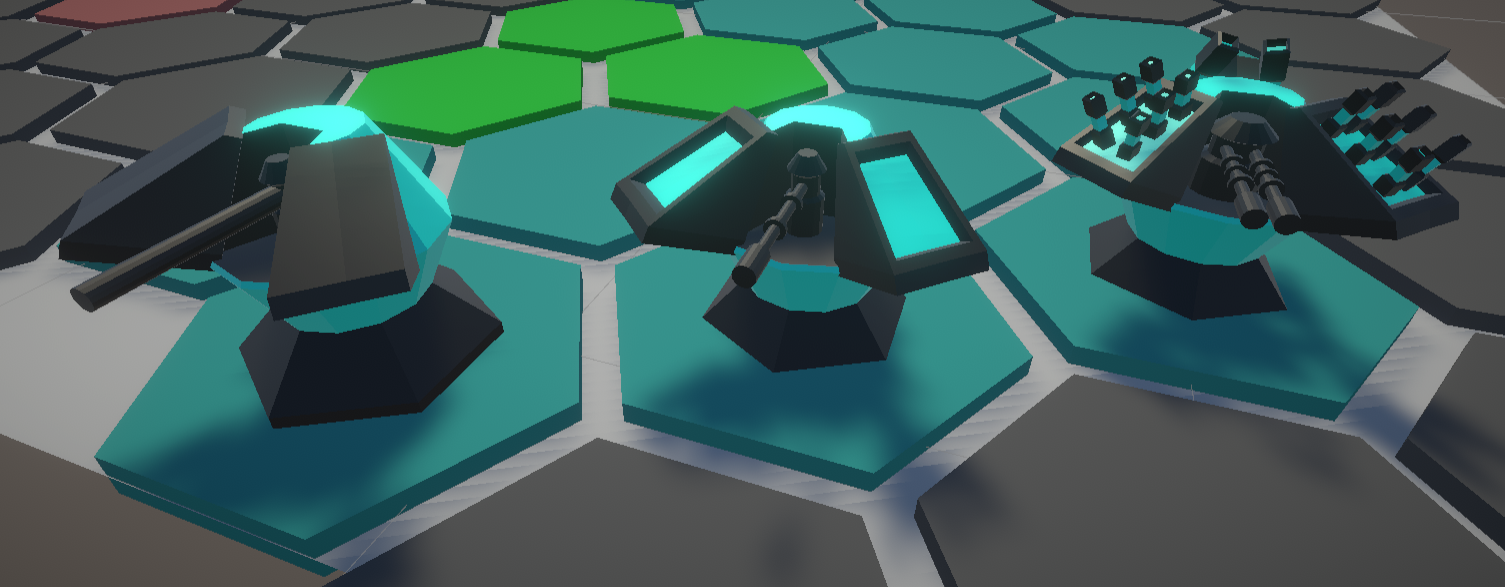
\includegraphics[width=1\textwidth]{vulkan.png}
	%	\caption{Vulkan}
	%	\label{fig: vulkan}
	%\end{figure}

	%\begin{figure}[H]
	%	\centering
	%	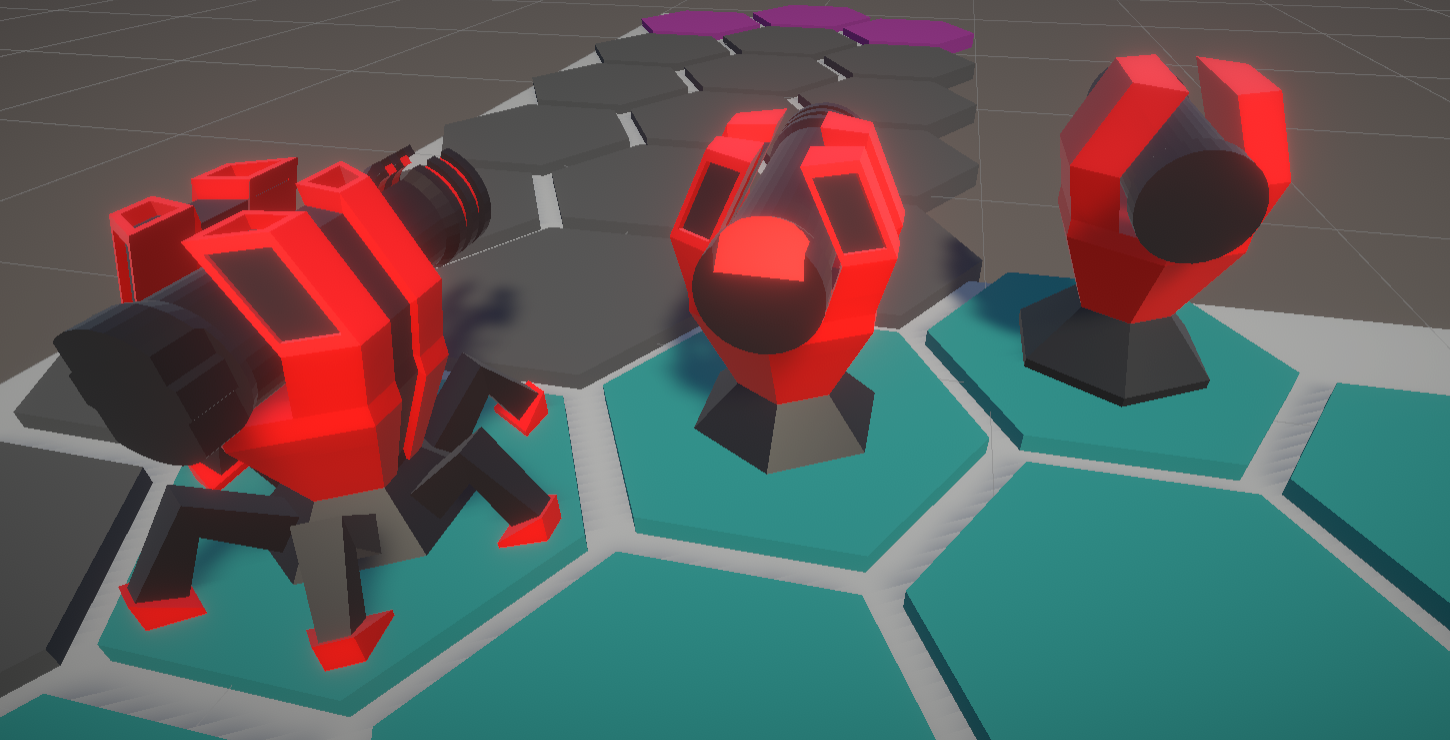
\includegraphics[width=1\textwidth]{machineCannon.png}
	%	\caption{Aruncatorul de flacari}
	%	\label{fig: machineCannon}
	%\end{figure}
	
	%\begin{figure}[H]
	%	\centering
	%	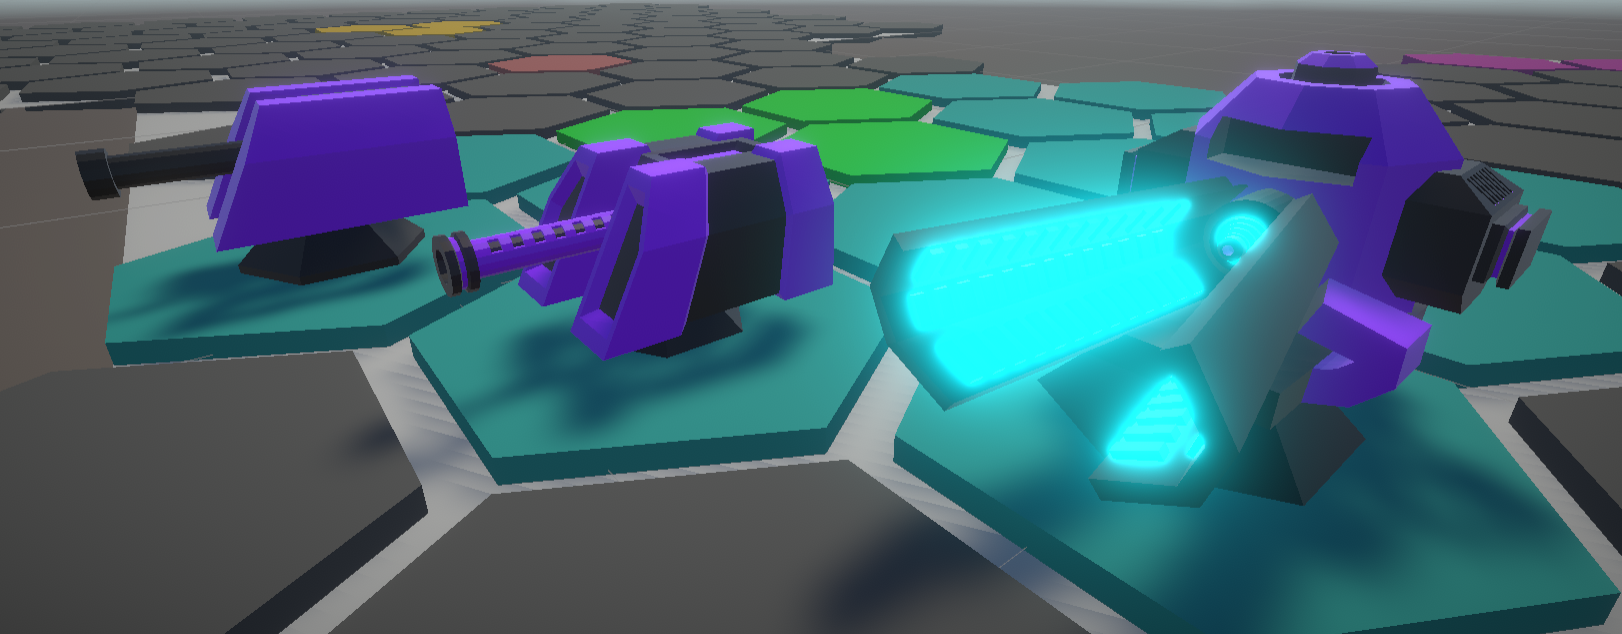
\includegraphics[width=1\textwidth]{railgun.png}
	%	\caption{Laser}
	%	\label{fig: railgun}
	%\end{figure}

	%\begin{figure}[H]
	%	\centering
	%	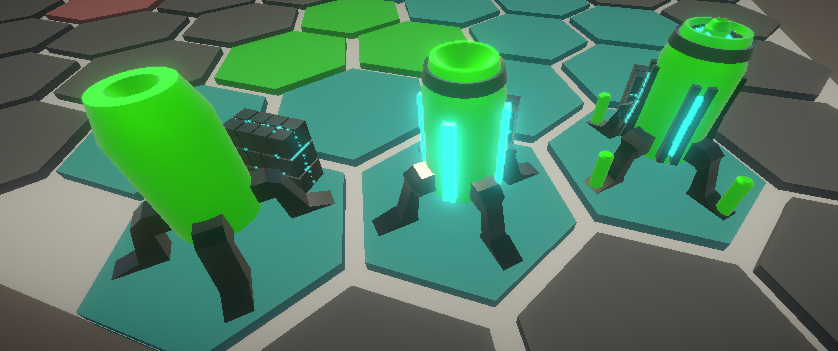
\includegraphics[width=1\textwidth]{excavator.png}
	%	\caption{Excavator}
	%	\label{fig: excavator}
	%\end{figure}
	
	
	
	
	
	\subsection{Sistemele Jocului}
	
	
	
	
	
	\subsubsection{Harta de joc}
	
	Pe hara jocului vor fi generate automat obiecte hexagonale. Aceste obiecte pot fi de mai multe tipuri:
	\begin{itemize}
		\item Hexagoane goale (cele gri din (fig: \ref{fig: gridSystem})).
		\item Hexagoane pe care putem construii turnuri de atac. (cele albastre din (fig: \ref{fig: gridSystem}))
		\item Hexagoane pe care putem construii turnul de extragere de resurse. (cele verzi din (fig: \ref{fig: gridSystem}))
		\item Hexagonul pe care va incepe si se va afla comandantul. (cel roz din (fig: \ref{fig: gridSystem}))
		\item Hexagoanele bazei. Baza va ocupa 3 hexagoane de acest tip. (cele galbene din (fig: \ref{fig: gridSystem}))
		\item Hexagonul ocupat. Fiecare hexagon care este ocupat de o anumita structura devine un astfel de hexagon. (are culoarea rosie)
	\end{itemize}

	Inamicii vor calcula drumul pe care merg in functie de toate aceste tipuri de hexagoane. Din acest motiv este nevoie si de cel gol.
	
	%\begin{figure}[H]
	%	\centering
	%	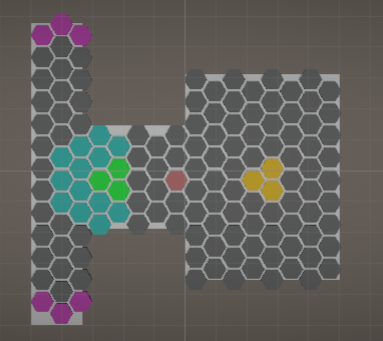
\includegraphics[width=1\textwidth]{grid.png}
	%	\caption{Harta de joc}
	%	\label{fig: gridSystem}
	%\end{figure}


	
	
	
	\subsubsection{Sistemul Turnurilor}
	
	Turnurile pot fi plasate doar pe hexagoanele de constructie. Odata plasate, acestea nu pot fi mutate. Singurele metode de a goli acel hexagon sunt sa fie distrus de un inamic sau sa vindem tureta respectiva. Daca vindem o tureta, vom primii inapoi o parte din banii investiti, bani cu care putem sa imbunatatim turnurile. Toate turnurile au urmatoarele proprietati:
	\begin{itemize}
		\item Viteza de atac
		\item Putere de atac
		\item Viata
		\item Raza de atac
		\item Inamicii pe care pot sa ii atace
	\end{itemize}

	Daca viata turetei ajunge la 0, va fi distrusa automat. Atata timp cat o tureta nu este distrusa, o putem repara, dar reparatiile vor fi executate intr-un anumit timp, iar in acest timp, tureta nu va putea sa atace dar poate sa fie atacata in continuare.
	
	
	
	
	
	\subsubsection{Comandantul}
	
	Comandantul poate fi mutat pe orice hexagon care nu este deja ocupat. Dupa ce ai ales un hexagon, acesta va incepe sa se miste catre acesta. Cat timp este in miscare, nu poate ataca inamicii. Destinatia poate fi schimbata doar dupa ce a ajuns la destinatie. Are raza medie, rata de atac medie, putere de atac mediu si poate ataca orice tip de inamic. Acesta poate intra si in turete, imbunatatindu-le exponential.
	
	
	
	
	
	\subsubsection{Valul de inamici}
	
	Jocul va avea mai multe nivele, care pot fi selectate dintr-un meniu, acestea fiind cat mai diversificate posibil. Inamicii au mai multe puncte din care pot sa vina in functie de nivelul ales. Acestia vin in grupuri de inamici. Intre fiecare grup exista o perioada de repaus in care jucatorul isi poate repara turnurile. In caz ca nu are nevoie de reparatii, poate selecta sa sara peste perioada de repaus, astfel primind bani extra.
	
	
	
	
	
	\subsubsection{Nivelele jocului}
	
	Nivelul este terminat cand toti inamicii au fost omorati. Fiecare nivel va avea un scor de maxim 3 stele, care specifica cat de bine s-a descurcat la acest nivel. Scorul este calculat in functie de viata ramasa a bazei la finalul nivelului. Fiecare stea castigata va da bani extra, bani care pot fi folositi in magazinul de imbunatatiri permanente, despre care vom discuta in scurt timp.
	\newline
	
	Jucatorul poate sa joace din nou nivelele, dar nu va mai primii atat de multi bani ca prima data. Acesta va castiga bani extra de pe stelele castigate doar daca a primit mai multe stele decat turele anterioare.
	
	
	
	
	
	\subsubsection{Lock-on}
	
	Jucatorul poate sa apese pe inamici, astfel setand acel inamic drept o prioritate. Fiecare turn care poate ataca acest tip de inamic il va prioritiza fata de alti inamici. De indata ce este omorat, se pierde aceasta prioritate.
	
	
	
	
	
	\subsubsection{Magazinul de imbunatatiri permanente}
	
	Intre nivele putem sa cumparat piese de schimb pentru turnurile noastre pentru a le face mai puternice. Aceste piese se pot cumpara doar cu banii castigati de pe urma nivelelor. Imbunatatirile pt fiecare tureta in parte sunt urmatoarele:
	
	\begin{itemize}
		\item Mitraliera automata: atac mai puternic, raza de atac mai mare, costuri mai mici.
		\item Gardul electric: mai multa viata, atac mai puternic, costuri mai mici.
		\item Vulkan: atac mai puternic, range mai mare, atac mai rapid
		\item Aruncatorul de flacari: atac mai puternic, range mai mare
		\item Laser: atac mai puternic, range mai mare
		\item Excavator: da bani mai multi, timpul intre livrarile de bani mai scurt
	\end{itemize}
	
	Fiecare imbunatatire va avea mai multe nivele, fiecare costand din ce in ce mai multi bani, dar vor avea un nivel maxim la care putem duce aceste imbunatatiri.
	
	
	
	
	
	\subsubsection{Raid system}
	
	Cand un jucator alege acest mod, este dus la o pagina de login in care trebuie sa isi specifice numele sau sa il lase pe cel generat automat. Dupa ce intra in cont, trebuie sa intre intr-un lobby. Ca sa intre intr-unlobby poate sa creeze el un lobby, sa aleaga un lobby dintr-o lista cu toate lobby-urile existente sau sa intre automat intr-un lobby existent. In cazul ultimei optiuni, in caz ca nu exista nici un lobby, acesta se creeaza automat. La aceasta pagina poate sa selecteze dificultatea nivelului si daca coechipierul este pregatit. De indata ce amandoi jucatorii sunt gata, pot sa inceapta nivelul.
	\newline
	
	In centrul mapei se afla un monstru imens de foc. Scopul nivelului este sa invingi monstrul impreuna cu coechipierul tau, inainte ca monstrul sa distruga baza vreunuia dintre jucatori.
	\newline

	Fiecare jucator poate plasa turnuri oriunde, putand sa imbunatateasca, repare sau vinde doar turnurile construite de ei. Amandoi playerii au caracterele lor comandant, dar acestia nu pot intra in aceeasi tureta in acelasi timp. Pentru sistemul de lock-on, doar turnurile jucatorului care a setat lock-on-ul va ataca inamicul prioritizat.
	
	
	
	
	
	\subsubsection{Atacurile monstrului de foc}
	
	Monstrul de foc are o serie de atacuri predefinite care devin mai puternice in dificultatile avansate.
	
	\begin{itemize}
		\item Abilitate automata: creste puterea de atac pe masura ce pierde din viata
		\item Ploaia de meteoriti: ridica o mana sus si genereaza meteoriti unul dupa altul. Fiecare meteorit cand este construit complet alege un turn si porneste catre directia acestuia. Cand se izbeste de turn explodeaza si scade din viata turnului in functie de dificultatea selectata.
		\item Gheara invartitoare: se invarte 360 grade si loveste toate turnurile de pe harta cu mana lui dreapta.
		\item Meteoritul suprem: cand ajunge la un anumit procentaj de viata incepe acest atac. Alege una dintre bazele jucatorilor (in caz ca sunt mai multi), se roteste spre ea si incepe sa incarce un meteorit imens. Incarcarea acestuia dureaza 30 de secunde. Daca in acest timp jucatorul reuseste sa ii scada suficient de mult viata monstrului, atacul este intrerupt si el devine confuz timp de 10 secunde, timp in care poate fi atacat neintrerupt. Daca jucatorii nu reusesc sa ii scada suficient de mult viata, va lovii puternic cu meteoritul baza selectata si turetele de prin jur.
	\end{itemize}

	Toate interactiunile acestui nivel sunt sincronizate in retea prin utilizarea Photon Engine-ului.
	
	
	
	
	
	\subsection{Analiza proiectului din punctul de vedere al consumatorilor}
	
	
	
	
	
	\subsubsection{Dificultatea jocului}
	
	Jocul va fi relativ dificil. Jucatorul trebuie sa se gandesca unde sa construiesca anumite turnuri pentru a folosi resursele cat mai bine. La inceput jocul va fi usor, dar pe masura ce progreseaza, nivelele vor devenii din ce in ce mai dificile. Trebuie sa se gandesca si daca poate rezista sa sara peste perioada de repaus intre grupurile de inamici.
	\newline
	
	Raid system-ul are un nivel de dificultate cu mult mai ridicat, pentru ca trebuie sa se gandeasca cum sa se coordoneze cat mai bine cu coechipierul.
	
	
	
	
	
	\subsubsection{Elemente de dependenta}
	
	In caz ca nu putem depasii un anumit nivel, putem juca nivelele anterioare si sa ne asiguram ca luam 3 stele la fiecare nivel. Aceasta metoda de a obtine 3 stele la fiecare nivel poate fi unul din motivele care ii determina pe jucatori sa continue sa joace jocul. Un alt factor ar putea fi sistemul de imbunatatiri permanente.
	
	
	
	
	
	\subsubsection{Grupele de varsta vizate}
	
	Acest joc nu are limitari de varsta, poate fi jucat de oricine, dar va fi apreciat cel mai mult de copii si de adolescentii care cauta provocari in jocurile de strategie. Jocul este in principiu facut pentru "casual gamers".
	
	
	
	
	
	\section{Implementare proiect}
	
	
	
	
	
	\subsection{Scena de lupta}
	
	
	
	
	
	\subsubsection{Initializarea scripturilor}
	\label{section: initialization}
	
	In Unity scripturile au cateva metode care ajuta la initializare.
	\newline
	
	\textbf{Awake} este metoda care este apelata la inceputul programului si inainte de restul metodelor.
	\newline
	
	\textbf{Start} este metoda care este apelata dupa ce au fost apelate metodele "Awake" de la toate scripturile.
	\newline
	
	\textbf{Update} este apelat la fiecare cadru al jocului, aici intervenind o mare parte din logica jocurilor. Apelarea update-ului incepe dupa ce toate metodele "Start" au fost apelate.
	\newline
	
	Pentru "Start" si "Awake", unity decide automat in ce ordine sa le apeleze, fara ca noi sa putem controla acest lucru. In multe proiecte mai complexe se ajunge in momentul in care, pentru initializatea anumitor sisteme este necesar ca alte sisteme sa fie deja initializate. Cum nu putem controla ordinea de initializare, se ajunge in punctul in care putem primi erori aleatorii din cauza initializarii haotice.
	\newline
	
	Pentru a combate acest lucru, m-am gandit la un sistem care va permite controlarea initializarii tuturor acestor procese cu usurinta.
	
	%\begin{figure}[H]
	%	\centering
	%	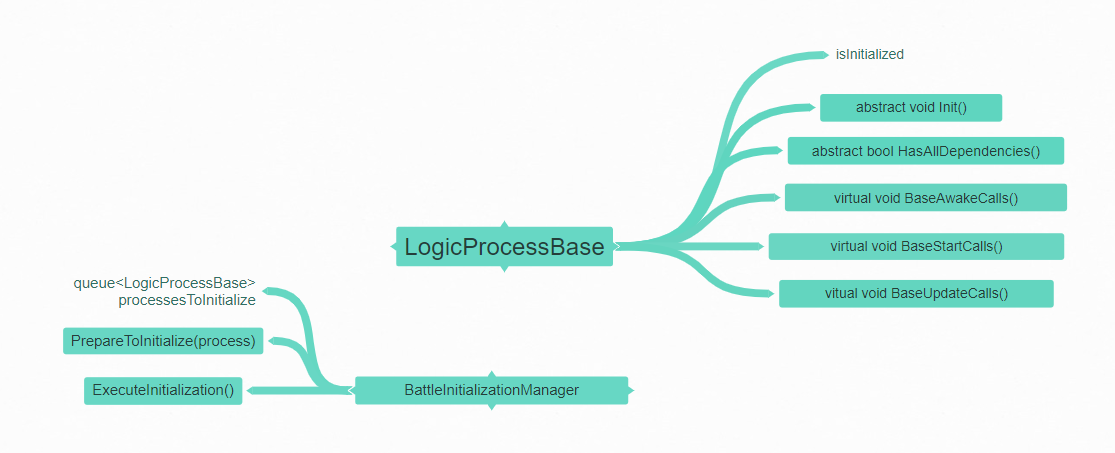
\includegraphics[width=1\textwidth]{logicProcessCoggle.png}
	%	\caption{Initializarea scripturilor}
	%	\label{fig: logicProcessCoggle}
	%\end{figure}
	
	Am creat clasa LogicProcessBase care ajuta in acest proces. Fiecare script care necesita o initializare mai organizata trebuie sa o mosteneasca. Aceasta contine:
	\begin{itemize}
		\item \textbf{isInitialized} care specifica daca scriptul curent a fost initializat sau nu inca
		\item \textbf{Init()}. In aceasta metoda trebuie sa scriem tot codul de initializare a clasei care mosteneste.
		\item \textbf{HasAllDependencied()}. Este o metoda care returneaza un boolean. In aceasta clasa trebuie sa punem toate dependintele de care are nevoie clasa care mosteneste.
		\item \textbf{BaseAwakeCalls()}. In aceasta metoda apelam "PrepareToInitialize()" din clasa "BattleInitializationManager", despre care vom vorbi in scurt timp.
		\item \textbf{BaseStartCalls()} si \textbf{BaseUpdateCalls()} sunt metode in care trebuie sa scriem tot codul care normal ar fi venit in Start/Update. In unity, nu putem defini Start/Update drept virtual si sa modificam functiile lor pe urma, din acest motiv tot codul din clasele dintr-o ierarhie mai complexa trebuie sa fie scris in aceste metode, iar in clasa cel mai jos din ierarhie trebuie sa le apelam in Awake/Start/Update.
	\end{itemize}

	\textbf{BattleInitializationManager} este a doua clasa de care avem nevoie. Ea este responsabila pentru a executa initializarea propriuzisa a proceselor. 
	\newline
	
	\textbf{PrepareToInitialize()} este apelata de fiecare proces in metoda lor de awake, iar aceasta metoda va adauga procesul intr-o coada.
	\newline
	
	\textbf{ExecuteInitialization()} parcurge toate procesele din coada si verifica daca acestea pot fi initializate, apeland "HasAllDependencies()". Daca procesul curent poate fi initializat, atunci apeleaza metoda "Init()" si seteaza "isInitialized = true". Daca nu il poate initializa, il adauga la finalul cozii pentru a fi initializat la final. Acest proces se repeta pana cand coada este goala sau s-a parcurs o data coada cap-coada si nu s-a initializat nici un proces. In acest caz inseamna ca aveau dependinte circulare si oprim procesul de initializare, afisand un mesaj de eroare. Aceasta metoda trebuie apelata in Awake, Start si Update, deoarece, pe parcurs pot aparea noi procese care trebuie initializate, iar programul trebuie sa poata sa detecteze astfel de cazuri.
	
	
	
	
	
	\subsubsection{Procesarea comenzilor venite de la utilizator}
	
	O alta problema des intampinata in proiectele mari este procesarea comenzilor venite de la utilizator. In cazul in care procesam comenzile in mai multe script-uri, cand vrem sa schimbam modul in care functioneaza comenzile sau sa schimbam platforma pe care ruleaza jocul, va trebuii sa schimbam toate scripturile in care procesam comenzile utilizatorului. In proiectele mari, acest lucru duce la mult timp pierdut si din acest motiv m-am gandit la o metoda cum sa imi organizez mai bine acest sistem.
	\newline
	
	Ideea propusa de mine este sa pastram toata procesarea de comenzi ale utilizatorului intr-un singur script. Acest script are definite evenimente/delegate pentru toate tipurile de input specifice. Alte scripturi se pot abona la aceste evenimente, iar cand utilizatorul apasa tasta respectiva, toate metodele abonate la evenimentul respectiv vor fi apelate.
	\newline
	
	Pe langa asta, este necesar sa stim si anumite informatii legate de comanda primita la utilizator. Informatiile aditionale de care am avut nevoie sunt:
	
	\begin{itemize}
		\item Pozitia pe ecran la care a fost apasat mouse-ul/ecranul (in cazul rularii pe android)
		\item Pozitia pe ecran la care a fost ridicata apasarea mouse-ului/ecranului (in cazul rularii pe android)
		\item Daca in clipa curenta este sau nu apasat mouse-ul/ecranul
		\item Timpul la care a fost apasat mouse-ul/ecranul
		\item Timpul la care a fost ridicata apasarea mouse-ului/ecranului
		\item Obiectul pe care utilizatorul a dat click in scena. In momentul cand apasam click, se creeaza un Raycast care are ca origine pozitia mouse-ului pe ecran si care se indreapta catre scena in perspectiva in care se afla camera la clipa curenta. Acest Raycast detecteaza daca a fost lovit un obiect, si daca da, retinem care obiect a fost lovit pt ca alte scripturi sa se poata folosi de aceasta informatie.
		\item Elementul cel mai de sus din ierarhia obiectului lovit. Datorita faptului ca anumite modele au o structura complexa, uneori nu ne este deloc util sa stim in mod direct ce obiect a fost lovit. De exemplu in caz ca apasam peste un turn si Raycast-ul loveste pusca turnului, nu ne va ajuta deloc in cazul in care ne intereseaza sa aflam ce tip de turn am lovit. Din acest motiv, in clipa in care gasim obiectul pe care am dat click, retinem si parintele cel mai de sus din ierarhie.
	\end{itemize}

	Aceasta organizare a procesarii comenzilor ne permite sa schimab tastele folosite cu usurinta si sa adaugam suport pentru dispozitive noi foarte usor. In cazul dispozitivelor noi, putem folosi directive de unity pentru a separa codul specific pentru calculator de cel specific pentru android sau orice alt dispozitiv. Procesarea comenzilor in cele 2 cazuri vor fi diferite, dar datorita faptului ca se invoca evenimentele deja devinite, alte script-uri nu trebuie modificate absolut deloc.
	
	
	
	
	
	\subsubsection{Harta de joc}
	
	Actiunea jocului se petrece pe o harta care este formata din mai multe blocuri hexagonale. Aceasta harta este generata automat in functie de ce tip de harta alegem pentru nivelul respectiv. Inainte sa incepem sa investigam indetaliat sistemul hartii de joc, trebuie mai intai sa definim ce reprezinta un bloc hexagonal pe harta.
	\newline
	
	
	
	
	
	\textbf{Blocul hexagonal}
	
	Pentru a retine informatii specifice pentru un bloc, am definit clasa HexagonalBlock. In interiorul clasei m-am folosit de doua enum-uri: SpawnPointsID si HexagonType.
	\newline
	
	HexagonType defineste tipul blocului hexagonal si interactiunile posibile cu acesta. Tipurile definite in acest enum sunt:
	
	\begin{itemize}
		\item Walkable. Blocul primeste culoarea gri si toate creaturile pot sa se deplaseze pe acesta.
		\item TurretBuildable. Blocul primeste culoarea albastra si reprezinta zonele de pe harta unde putem sa construim turnurile noastre.
		\item ResourceExtraction. Blocul primeste culoarea verte si reprezinta zonele de pe harta in care putem construii turnul excavator.
		\item Occupied. Blocul primeste culoarea rosie si reprezinta zonele in care este construita un turn sau locul in care se afla comandantul.
		\item SpawnPoint. Blocul primeste culoarea mov si reprezinta locul din care pornesc inamicii.
		\item Impassable. Blocul primeste culoarea rosu inchis si reprezinta locurile prin care nu pot sa treaca inamicii. Sistemul de navigare va ignora toate aceste blocuri si va gasi rute alternative.
		\item PlayerBase. Blocul primeste culoarea galbena si reprezinta locul in care va fi creata baza jucatorului. Pentru ca un nivel sa fie considerat valid, trebuie sa existe 3 astfel de blocuri unul langa altul.
		\item CommanderSpawn. Blocul primeste culoarea mov si reprezinta locul in care va incepe comandantul. Pentru ca un nivel sa fie considerat valid, trebuie sa existe exact o instanta a acestui bloc pe harta.
	\end{itemize}
	
	SpawnPointsID defineste o serie id-uri pentru blocurile de tip SpawnPoint. In fisierul de configurare al valului de inamici, discutat in capitolul \ref{section: enemyWave}, putem specifica id-ul blocului de la care vor incepe inamicii. In caz ca, pentru un val de inamici specificam ca inamicii sa incepa de la o locatie aleatorie, atunci se va alege un bloc aleatoriu dintre toate blocurile de pe harta.
	\newline
	
	Blocul hexagonal defineste si o lista de materiale, care sunt folosite pentru a schimba culoarea blocului in momentul in care tipul acestuia se schimba.
	\newline
	
	Are definite si 2 metode ajutatoare si anume PlaceHexagon(), care aseaza blocul pe harta in functie de pozitia si diametrul specificat in parametrii, si UpdateMaterial() care actualizeaza culoarea blocului, prin schimbarea materialului pe care il foloseste.
	\newline
	
	Pentru a pune in functiune schimbarea de culoare a blocului hexagonal direct din editor, a trebuit sa creez clasa speciala HexagonalBlockEditor. Aceasta clasa mosteneste clasa Editor, pentru a putea schimba interfata grafica a editorului din Unity. Aceasta clasa, in metoda OnInspectorGUI care este apelata de fiecare data cand obiectul este selectat, verifica daca s-a schimbat tipul blocului, si daca da, atunci apeleaza metoda UpdateMaterial() de pe blocul selectat.
	\newline
	
	
	
	
	
	\textbf{Harta propriu-zisa}
	
	Clasa special definita pentru harta de joc este HexagonalGrid. Aceasta clasa are cateva proprietati publice care definesc dimensiunea hartii: diameter (care defineste cat de mare este fiecare hexagon), offset (care este aplicat in asa fel incat hexagoanele vor fi pozitionate la distante egale intre ele) si mapScaleOffset (harta de joc este scalata automat la dimensiunea ecranului; acest offset ne ajuta sa scalam harta mai mult sau mai putin decat ar fi fost scalata automat).
	\newline
	
	Scriptul are definit o lista de tipul HexagonalBlock, care retine toate blocurile hexagonale de pe harta si mai are definit o variabila publica care reprezinta tipul de harta pe care o folosim. Tipul de harta este reprezentat de un model 3D care va fi folosit pentru a pozitiona hexagoanele.
	\newline
	
	Clasa mosteneste LogicProcessBase, iar in metoda init, gaseste fisierul de configurare al nivelului curent, discutat in capitolul \ref{section: stageScriptable}, sterge toate blocurile existente de pe harta, citeste fisierul de configurare al hartii (definit in fisierul de configurare al nivelului si explicat in sectiunea urmatoare). Dupa ce a citit continutul fisierului, apeleaza metoda SpawnAndScaleMap() si metoda LoadPresetGrid().
	\newline
	
	SpawnAndScaleMap() creeaza o instanta a hartii de joc (modelul 3d care este definit drept variabila publica), gaseste limitele acesteia in coordonate 3D, si in functie de dimensiunea ecranului, scaleaza harta in asa fel incat sa incapa harta in intregime pe ecran. Pe urma, in functie de mapScaleOffset, scaleaza din nou harta in functie de dorinta persoanei care a definit nivelul.
	\newline
	
	Inainte sa vorbim despre functia LoadPresetGrid() trebuie sa discutam despre CreateGrid(). Aceasta functie se foloseste de modelul 3D al hartii pentru a genera si pozitiona toate blocurile hexagonale necesare. Aceasta parcurge intreaga dimensiune a modelului 3D, si folosindu-se de fizica definita de unity (Physics.Raycast), verifica daca in pozitia curenta de pe model a reusit sa loveasca suprafata. In caz ca a reusit sa loveasca, atunci genereaza un bloc hexagonal, il adauga in lista si cauta in continuare pana cand a reusit sa parcurga intreg modelul 3D. La final o sa avem generate pe harta blocuri hexagonale care sunt pozitionate in toate zonele de pe modelul 3D al hartii, fiecare bloc fiind de tipul Walkable.
	\newline
	
	LoadPresetGrid() preia continutul fisierului configurabil, apeleaza metoda CreateGrid(), dupa care incepe sa itereze peste fiecare element din blocurile generate. La fiecare iteratie, initializeaza blocul curent in functie de datele din fisierul configurabil al hartii de joc, si in caz ca intalneste blocuri de tipul PlayerBase sau CommanderSpawn, genereaza si pozitioneaza pe harta comandantul si baza jucatorului. In caz ca fisierul este corupt, nu a gasit blocurile pentru comandant si penrtu baza jucatorului sau a gasit prea multe din acestea, afiseaza mesaje de eroare pentru fiecare caz in parte.
	\newline
	
	
	
	
	
	\textbf{Fisierul de configurare pentru harta de joc}
	
	Pentru a putea crea cu usurinta nivele cat mai variate, trebuie sa retinem anumite date in fisiere configurabile. Aceste fisiere configurabile trebuie sa fie facute in asa fel incat prin incarcarea unui simplu fisier, putem genera un nivel de joc complet functional.
	\newline
	
	In acest scop am definit clasa GridSaveData, care retine proprietaile cele mai importante ale hartii de joc. Aceasta clasa retine diametrul blocurilor, offset-ul si mapScaleOffset, pentru a putea incarca harta la aceeasi scala la care era configurata initial. Pe langa asta, retine o lista cu tipurile blocurilor hexagonale de pe harta si id-urile setate pentru blocurile de pe care incep inamicii.
	\newline
	
	Aceasta clasa este definita urmand o structura json, pentru a usura serializarea si deserializarea datelor in momentul scrierii si citirii pe disk.
	\newline
	
	Pe langa aceasta clasa, am avut nevoie si de o clasa ajutatoare care sa se ocupe de salvarea si incarcarea propriu-zisa a datelor. Clasa se numeste GridDataSaver si este definita cu 2 metode statice simple: SaveData() si LoadData().
	\newline
	
	
	
	
	
	\textbf{Editorul special pentru crearea rapida a nivelelor}
	
	Pentru a usura generarea de nivele, am creat un editor cu functii speciale. Clasa se numeste HexagonalGridEditor si mostenteste clasa Editor din Unity. Folosind aceasta clasa, am suprascris editorul implicit pentru clasa HexagonalGrid, iar in loc i-am adaugat cateva proprietati ajutatoare. Am definit campuri publice pentru modelul 3D al hartii pentru care dorim sa cream un nivel, diametru, offset, mapScaleOffset si locatia fisierului de configurare in care sa salveze configurarea hartii si din care poate sa incarce harta pentru a o modifica.
	\newline
	
	Pe langa aceste campuri, am definit si cateva butoane care au ca rol sa apeleze functionalitati din scriptul HexagonalGrid. Fara aceste butoane, nivele ar fi putut fi create numai in timpul rularii aplicatiei, fapt ce nu era de dorit, deoarece este cu mult mai usor sa cream harti de joc direct din editor. Butoanele definite sunt: Scale Map, Reset Scale, Generate Grid, Clear Grid, Load Preset, Save Preset. Fiecare buton apeleaza functionalitatea cu acelasi nume din HexagonalGrid, exceptant Load Preset si Save Preset, care incarca si salveaza configurarea actuala a hartii in locatia specificata prin campul public, folosindu-se de GridDataSaver.
	\newline
	
	Datorita acestui editor special, procesul de creare a hartilor jocului a devenit foarte rapid. Pentru a crea o harta noua, trebuie sa incarcam un model 3D simplist definit intr-un program de modelare 3D, tragem acel model 3D in campul public de pe editor. Modificam campurile de scalare a mapei si apasam pe butonul de Generate Grid repepat pana cand suntem multumiti de configurarea actuala. Dupa acest lucru, selectam blocurile hexagonale la care dorim sa le schimbam tipul. Datorita editorului HexagonalBlockEditor, culoarea acestora se schimba automat, fapt care ne usureaza munca enorm. Dupa ce am definit toate tipurile blocurilor, specificam locatia la care dorim sa salvam fisierul de configurare al hartii si apasam pe butonul Save Preset.
	\newline
	
	In caz ca dorim sa modificam configurarea unei harti, specificam locatia fisierului de configurare a hartii respective. Setam campul modelului 3D cu modelul 3D pe care a fost generata initial harta si apasam pe butonul Load Preset. Dupa ce harta s-a incarcat cu succes, putem modifica blocurile hexagonale in modul dorit, iar cand am terminat apasam din nou pe butonul Save Preset prentru a suprascrie configurarea hartii.
	\newline
	
	
	
	
	
	\subsubsection{Sistemul de navigare}
	
	Caracterele jocului trebuie sa stie pe unde pot sa mearga ca sa ajunga la o anumita destinatie. In acest scop a trebuit sa aleg un algoritm care sa gaseasca cel mai scurt drum posibil. Am avut de ales intre mai multi algoritmi specifici, precum: Dijkstra, A*, Floyd-Warshall, etc.
	\newline
	
	In cele din urma am ales sa folosesc Floyd-Wharshall. Acest algoritm are complexitatea $O(n^3)$ si presupune construirea celor mai scurte drumuri posibile pornind de la oricare nod catre oricare alt nod din retea. Deoarece construirea drumului se realizeaza doar la inceputul jocului si reconstruirea acestui drum se realizeaza aproape instantaneu, am ales sa folosesc acest algoritm.
	\newline
	
	"Consideram reteaua orientata $G = (N, A, b)$ reprezentata prin matricea valoare adiacenta $B = (b_{ij}), i, j \in N$ cu
	
	\begin{equation*}
		b_{ij} = \begin{cases}
			b(i, j) \quad daca \quad i \neq j \quad si \quad (i, j) \in A; \\
			0 \quad daca \quad i = j; \\
			\infty \quad daca \quad i \neq j \quad si \quad (i, j) \neq A.
		\end{cases}
	\end{equation*}

	Algoritmul Floyd-Warshall determina matricea distantelor $D = (d_{ij}), i, j \in N$ si matricea predecesor $P = (p_{ij}), i, j \in N$." \cite{grafuriAnul2}
	
	\begin{algorithmic}
		\Function{Floyd-Warshall}{}
			\For{i $\gets$ 1 to n}
				\For{j $\gets$ 1 to n}
					\State $d_{ij} \gets b_{ij};$
					\If{i $\neq$ j and $d_{ij} < \infty$}
						\State $p_{ij} = i;$
					\Else
						\State $p_{ij} = 0;$
					\EndIf
				\EndFor
			\EndFor
			
			\For{k $\gets$ 1 to n}
				\For{i $\gets$ 1 to n}
					\For{j $\gets$ 1 to n}
						\If{$d_{ik} + d_{kj} < d_{ij}$}
							\State $d_{ij} = d_{ik} + d_{kj};$
							\State $p_{ij} = p_{kj};$
						\EndIf
					\EndFor
				\EndFor
			\EndFor
		\EndFunction
	\end{algorithmic}

	\begin{algorithmic}
		\Function{Reconstruire Drum}{}
			\State k = n;
			\State $x_k = j$
			\While{$x_k \neq i$}
				\State $x_{k - 1} = p_{ix_k};$
				\State k = k - 1
			\EndWhile
		\EndFunction
	\end{algorithmic}

	Drumul minim este $D_{ijp} = (x_k, x_{k+1}, \dots, x_{n-1}, x_n) = (i, x_{k+1}, \dots, x_{n-1}, j)$
	
	
	
	
	
	\subsubsection{Interfete folosite}
	
	Pentru ca o serie de obiecte din joc trebuie sa urmeze aceleasi concepte, am decis sa ma folosesc de interfete pentru a le definii modul in care trebuie sa functioneze. 
	\newline
	
	\textbf{IMovable}
	
	Deoarece inamicii si comandantul se pot misca pe mapa, am definit aceasta interfata pentru a defini aceleasi concepte pentru toate caracterele care au nevoie de a se misca pe mapa. Interfata se foloseste de sistemul de navigare definit anterior si contine urmatoarele:
	
	\begin{itemize}
		\item Nodul curent la care se afla
		\item Nodul destinatie
		\item Nodul urmator la care trebuie sa se mute ca sa se apropie de destinatie
		\item Viteza de deplasare
		\item Distanta fata de urmatorul nod pt care consideram ca am ajuns la acesta. Deoarece lucram cu obiecte in spatiu 3D, este nevoide de o asemenea valoare.
		\item Un boolean care defineste daca am ajuns sau nu la destinatie
		\item O metoda care seteaza nodul urmator la care trebuie sa ajungem ca sa ne apropiem de destinatie. Acesta face apel la matricea construita de sistemul de navigare.
		\item O metoda care misca propriuzis obiectul catre urmatorul nod
		\item O functie care verifica daca am ajuns sau nu la destinatie.
	\end{itemize}
	\bigskip


	\textbf{IAttacker}
	
	 Este o interfata pe care toate obiectele/caracterele care vor sa atace alte obiecte trebuie sa o mostendeasca. Aceasta contine urmatoarele:
	 
	 \begin{itemize}
	 	\item Obiectul pe care trebuie sa il atace. Tipul este definit la mostenirea clasei datorita sablonului definit pentru interfata.
	 	\item Puterea de atac
	 	\item Raza de atac
	 	\item Durata intre atacuri
	 	\item Timpul la care s-a executat ultimul atac
	 	\item Intervalul de timp intre care se cauta un nou inamic
	 	\item Metoda care afisaza/ascunde raza obiectelor din scena. Raza acestora a fost defnita intr-un shader special creat in Shader Graph
	 	\item O metoda care cauta cel mai apropiat inamic daca exista in raza
	 	\item Metoda de atac pe care fiecare obiect o implementeaza diferit.
	\end{itemize}
 	\bigskip
 	
 	\textbf{IDestroyable}
 	
 	Fiecare obiect care are o viata anume si care poate fi distrus trebuie sa mosteneasca aceasta interfata. Aceasta contine urmatoarele:
 	
 	\begin{itemize}
 		\item Viata obiectului.
 		\item Banii primiti cand obiectul este distrus
 		\item O metoda care distruge obiectul respectiv cand viata lui a ajuns la 0
 	\end{itemize}
 	\bigskip
 	
 	\textbf{IRecoverable}
 	
 	Turnurile pot sa isi refaca viata, iar ca un concept pentru viitor, ar putea sa existe si anumiti inamici care refac viata altor inamici. Interfata contine urmatoarele:
 	
 	\begin{itemize}
 		\item Cata viata se reface in fiecare secunda cand efectul este aplicat.
 		\item Costul refacerii in cazul in care este de dorit un cost.
 		\item Un boolean care verifica daca se reface sau nu in clipa curenta.
 		\item O metoda care porneste procesul de refacere
 	\end{itemize}
	
	
	
	
	
	\subsubsection{Ierarhia inamicilor}
	
	%\begin{figure}[H]
	%	\centering
	%	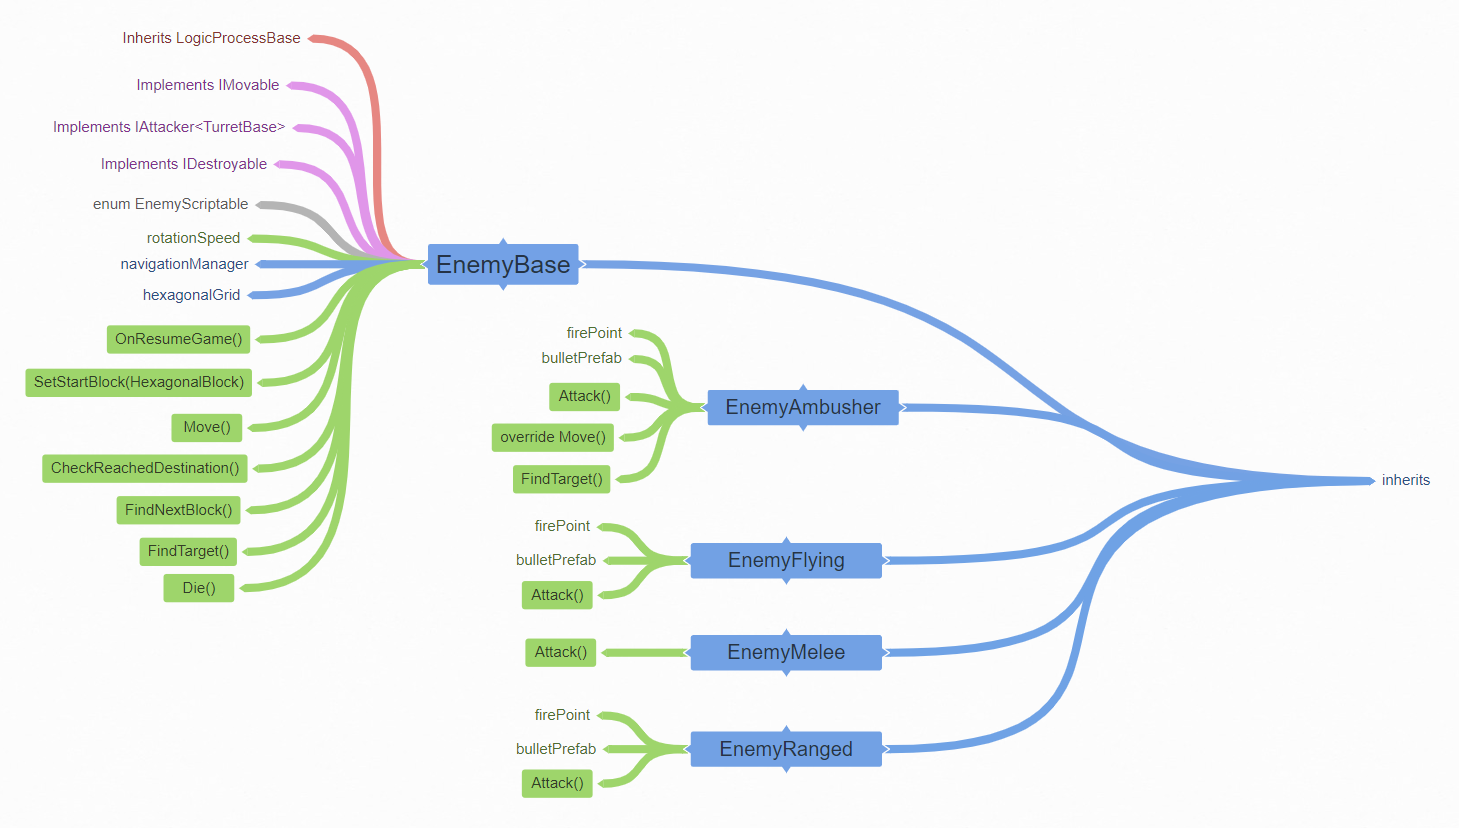
\includegraphics[width=1\textwidth]{EnemyHierarchy.png}
	%	\caption{Ierarhia inamicilor}
	%	\label{fig: enemyHierarchy}
	%\end{figure}

	In \ref{fig: enemyHierarchy} am definit intr-un mod simplu si colorat modul in care trebuie structurata ierarhia inamicilor din joc.
	\newline
	
	Clasa EnemyBase este clasa parinte care defineste modul principal in care inamicii trebuie sa functioneze. Aceasta clasa implementeaza 3 interfete utile, si anume IMovable, IDestroyable si IAttacker$\textless$TurretBase$\textgreater$. Precum am explicat si anterior, interfata IAttacker defineste un sablon care specifica tipul de obiect pe care poate sa il atace, in cazul nostru, clasa TurretBase care va fi explicata in urmatoarea sectiune.
	\newline
	
	Aceasta clasa face referire si la sistemul ne navigare si la sistemul hartii hexagonale, si din acest motiv este nevoie sa isi faca initializarea doar dupa ce aceste doua sisteme si-au terminat initializarea lor. In acest scop, putem sa mostenim clasa LogicProcessBase, care a fost descrisa in capitolul \ref{section: initialization}.
	\newline
	
	Functiile implementate de aceasta clasa sunt in mare parte functiile mostenite dupa implementarile interfetelor descrie, cu cateva exceptii referitoare la alte sisteme din joc. Un astfel de sistem este cel de a pune pe pauza jocul. Can jocul este pus pe pauza, toate scripturile care se foloseau de timpul actual al jocului nu vor actiona in modul asteptat dupa ce reluam jocul. Din acest motiv este nevoie sa implementam functia OnResumeGame() care va fi apelata cand se reia jocul, iar in aceasta functie trebuie sa setam toti temporizatorii din script la valorile necesare.
	\newline
	
	Aceasta clasa nu este suficienta pentru a definii toate tipurile de inamici, deoarece face dificila diferentierea intre inamici pentru anumite sisteme si anumiti inamici actioneaza diferit fata de standard. Din acest motiv este necesar sa definim o serie de clase pentru fiecare inamic in parte, care sa mosteneasca aceasta clasa de baza, si care sa isi adauge propia lor logica la standardul definit de EnemyBase.
	\newline
	
	\textbf{EnemyAmbusher} nu se foloseste de sistemul de navigare. Este inamicul bombardier, care zboara prin aer direct catre baza jucatorului. Cand ajunge in contact cu aceasta, lanseaza bombe care provoaca multe pagube, dupa care isi continua drumul, parasind scena de lupa. Din acest motiv metodele Move() si FindTarget() trebuie sa fie suprascrise.
	\newline
	
	\textbf{EnemyFlying} si \textbf{EnemyRanged} sunt inamici care urmeaza in totalitate logica definita de EnemyBase. Singura exceptie la aceste doua clase este ca anumite turnuri vor face diferentiere intre ele. O parte din turnuri pot sa atace doar inamicii de sol (EnemyRanged si EnemyMelee) iar alte turnuri pot sa atace doar inamicii zburatori (EnemyFlying si EnemyAmbusher).
	\newline
	
	\textbf{EnemyMelee} este un inamic care sa atace alte turnuri doar cand a ajuns langa turnuri. Din acest motiv metoda lui de atac trebuie sa fie suprascrisa putin.
	
	
	
	
	
	\subsubsection{Ierarhia turnurilor defensive}
	\label{section: turretHierachy}
	
	Ierarhia turnurilor este putin mai complexa si va fi descrisa pe bucati.
	
	\ \\
	\textbf{TurretBase}
	
	Urmand aceeasi logica ca la inamici, am definit o clasa de baza pentru modul in care trebuie sa actioneze un turn defensiv. Acesta implementeaza doua interfete: IDestroyable si IAttacker$\textless$EnemyBase$\textgreater$. Sablonul de la IAttacker defineste faptul ca un turn defensiv poate sa atace obiecte de tipul EnemyBase, care este clasa din care mostenesc toti inamicii jocului.
	\newline
	
	TurretBase are si ea nevoie de o initializare controlata si din acest motiv trebuie sa mosteneasca clasa LogicProcessBase. TurretBase defineste proprietatile turnurilor, cum ar fi viata, puterea de atac, etc. Pe langa asta, majoritatea turnurilor pot fi imbunatatine, proprietatile crescand exponential cand acest lucru se intampla. Din acest motiv a fost nevoie sa creez fisiere configurabile care definesc valori pt proprietatile turnurilor. Aceasta clasa detine o instanta a unui astfel de fisier, si defineste o functie "SetLevelProp(int level)" care citeste fisierul configurabil si seteaza toate proprietatile in functie de acesta. Pe langa asta, cand turnurile sunt imbunatatite, le schimba modelul 3D pentru a avea o schimbare vizuala.
	\newline
	
	Clasa defineste si alte metode care au fost abordate in capitolele anterioare, precum: Die(), OnResumeGame(), Init(), etc. Functia DrawRange() afiseaza/ascunde raza de atac a turnului, raza care a fost construita intr-un shader special definit in Shader Graph.
	
	\ \\
	\textbf{PlayerBase}
	
	PlayerBase este o clasa care mosteneste TurretBase, si reprezinta baza de operatii a jucatorului. Aceasta implementeaza o parte din actiunile definite in interfete, precum: Attack(), FindTarget(), etc.
	\newline
	
	Pe langa asta, cand baza jucatorului ramane fara viata si este distrusa, jocul trebuie sa se termine. Acest lucru poate fi realizat foarte usor prin suprascrierea metodei Die(). Cand baza ramane fara viata, instiinteaza managerul jocului, iar pe urma acesta isi porneste procesul de incheiere al nivelului. Mai multe detalii vor fi discutate in capitolul \ref{section: gameState}
	
	\ \\
	\textbf{BuildableTurret}
	
	BuildableTurret este clasa care mosteneste TurretBase si defineste functionalitatea pentru toate turnurile care pot fi construite pe harta de joc. Aceasta clasa implementeaza IRecoverable, care defineste modul in care turnurile pot sa isi refaca viata. De indata ce turnul a fost lovit de un inamic, se calculeaza un cost necesar pentru a readuce turnul la viata maxima. In caz ca jucatorul are suficienti bani si doreste sa refaca turnul, acesta va incepe procesul refacere. Pe parcursul catorva secunde, se va reface treptat pentru viata lipsa in momentul inceperii acestui proces. In acest timp turnul nu poate sa atace inamicii, dar poate sa fie lovit in continuare de acestia, deci nu este garantat ca va revenii la viata maxima dupa terminarea procesului.
	\newline
	
	O alta functionalitate majora a turnurilor este optiunea de a inbunatatii turnurile. Cand utilizatorul selecteaza un turn, se cauta in fisierul configurabil costul necesar pentru a imbunatatii turnul la nivelul urmator, in caz ca nu a ajuns inca la nivelul maxim. In caz ca jucatorul are suficienti bani se apeleaza metoda Upgrade(), care verifica daca s-a ajuns la nivelul maxim si daca nu, dezactiveaza toate starile defavorabile ale turnului (cum ar fi raza turnului), creste nivelul si apeleaza metoda SetLevelProp() pentru a citi din nou fisierul de configuratie pentru nivelul nou.
	\newline
	
	Turnul poate fi vantut de jucator in caz ca este in criza de bani sau vrea sa mute turnul in alta locatie. In acest caz se calculeaza banii pe care ii primeste jucatorul, se dezaciveaza toate starile si functionalitatile turnului si se distrug referintele specifice. Tote acestea se intampla in metoda SellTurret() implementata in aceasta clasa.
	\newline
	
	Ultima functionalitate adaugata de aceasta clasa este cea de a permite turnului sa fie controlat de comandantul jocului. Aceasta functionalitate va fi descria in detaliu in sectiunea \ref{section: commander} 
	
	\ \\
	\textbf{Turnurile specifice}
	
	Cel mai jos nivel din ierarhie presupune definirea claselor specifice pentru fiecare tip de turn in parte, fiecare dintre acestea mostenind clasa BuildableTurret si adaugand/modificand logica stabilita pana in acest punct in functie de caz.
	
	\begin{itemize}
		\item \textbf{TurretElectricFence}. Este turnul care are viata foarte mare dar raza de atac foarte mica. Poate sa atace doar inamicii de lupta apropiata si actioneaza drept un zid care pazeste toate celelalte turnuri de atacurile inamicilor. Aceast turn modifica functionalitatea prin care se gaseste ce inamic trebuie sa atace si modul in care ataca inamicul.
		\item \textbf{TurretExcavator}. Acest turn este cel mai diferit de norma, in sensul in care nu poate ataca deloc inamicii. Este un turn care la un anumit interval de timp farmeaza resurse, pe care le converteste la bani de joc. Din acest motiv a fost nevoie sa scape complet de cautarea inamicilor, iar metoda de atac a suprascris-o in functionalitatea de farmare de bani.
		\item \textbf{TurretFlamethrower}. De indata ce un inamic intra in raza acestui turn, lanseaza flacari violente in directia inamicului, flacari care ranesc toti inamicii care stau in ele. Turnul prioritizeaza inamicii de atac de aproape, dar in cazul in care nu exista astfel de inamici, ataca inamicii cu raza de atac. Nu poate sa atace inamicii zburatori sau cei bombardieri.
		\item \textbf{TurretMachineGun}. Este turnul universal care poate sa atace toti inamicii jocului. Acesta lanseaza gloante foarte rapid catre inamici, dar gloantele individual nu provoaca foarte multe daune. Fiecare nivel presupune o viteza de atac mai mare.
		\item \textbf{TurretLaser}. Acest turn ataca inamicii cu un laser foarte puternic care distruge compozitia moleculara a inamicului in fiecare clipa in care acestia sunt in raza turnului. Poate ataca inimacii de atac apropiat si cei de la distanta, dar ii prioritizeaza pe cei de la distanta. Nu poate ataca inamicii zburatori sau pe cei bombardieri.
		\item \textbf{TurretVulkan}. Este turnul special impotriva inamicilor zburatori si a celor bombardieri. Nu poate ataca inamicii de sol, dar in schimb lanseaza rachete catre cei zburatori, rachete care explodeaza cand ajung in contact cu acestia.
	\end{itemize}
	
	
	
	
	
	\subsubsection{Comandantul}
	\label{section: commander}
	
	Comandantul este un caracter special care poate fi miscat oriunde dorim pe harta si care ataca inamicii din raza lui de atac, cat timp nu se deplaseaza catre o noua locatie.
	\newline
	
	In acest scop, clasa Commander implementeaza interfetele IMovable si IAttacker$\textless$EnemyBase$\textgreater$. Comandantul nu poate sa fie distrus si din acest motiv nu este nevoia implementarii interfetei IDestroyable.
	\newline
	
	Comandantul are si el un fisier de configurare care specifica statusurile lui, cum ar fi viata, viteza de miscare, puterea de atac, etc. Pentru a se putea deplasa pe harta, are nevoie sa faca referire la sistemul de navigare si la cel al hartii de joc (grid system). Din acest motiv este necesar sa mosteneasca LogicProcessBase, ca sa isi execute initializarea doar dupa celelalte sisteme au reusit sa si-o termine pe a lor.
	\newline
	
	Majoritatea functiilor sunt similare cu cele ale turnurilor (Attack, DrawRange, FindTarget, etc.) asa ca nu vor fi reluate aici. 
	\newline
	
	Pe langa aceste functionalitati, comandantul poate sa intre in turnuri si sa le controleze, marindu-le astfel productivitatea. Cand acesta intra in turnuri, le mareste raza, viteza, puterea de atac si in cazul excavatorului de resurse, creste banii primiti la fiecare livrare de resurse. Ca sa poata intra in turnuri, trebuie sa se deplaseze la acel turn la comanda jucatorului, iar cand turnul este distrus/vandut, acesta iese din turn si se misca catre cel mai apropiat nod din graful hartii de joc care nu este deja ocupat. Comandantul poate sa iasa din turn si fara ca acesta sa fie dsitrus, dar acest lucru se intampla numai la comanda jucatorului.
	
	
	
	
	
	\subsubsection{Punerea pe pauza a jocului}
	
	Jucatorul are la dispozitie optiunea de a pune pe pauza jocul. Unity pune la dispozitie mai multe moduri de a pune pe pauza jocul. Unul din aceste moduri este de a modifica o variabila din clasa globala Time, si anume Time.timeScale. Aceasta variabila are in mod normal valoarea 1, dar daca o modificam toate sistemele jocului vor rula la o alta viteza. Daca ii setam o valoare de 0.5, majoritatea sistemelor vor incetinii (animatii, sisteme de particule, rata de apelare a metodelor update, etc.). In caz ca setam aceasta variabila la 0, toate sistemele care sunt depentende te timp se vor opri din a functiona pana cand se schimba aceasta variabila. 
	\newline
	
	Este o metoda valida de a crea un sistem care sa puna pe pauza jocul, dar deoarece opreste toate functiile update din a mai fi apelate si deoarece nu putem controla ce sisteme sunt oprite nu este o metoda folosita foarte des. Un motiv principal pt care nu este de recomandat aceasta solutie este pentru ca va opri inclusiv sunetele din joc, fapt ce nu este de dorit in cele mai multe cazuri.
	\newline
	
	O alta metoda de a implementa un sistem de pauza, este sa avem un script care tine referinte catre toate celelalte script-uri din scena si care, in momentul in care jucatorul pune pe pauza jocul, opreste scripturile dorite din a mai fi executate. Unity are o clasa speciala numita MonoBehaviour, care ne da toate functiile discutate anterior (Start, Update, Coroutine, OnTriggerEnter, etc.) si multe alte proprietati utile. Toate scripturile care mostenesc aceasta clasa pot fi puse pe obiecte 3D din scena, iar scripturile care nu implementeaza clasa MonoBehaviour nu pot fi puse pe obiecte din scena. Acestea din urma vor fi rulate numai cand cream obiecte de tipul acelor clase, sau in cazul claselor statice, cand apelam metode din ele. Clasele care mostenesc MonoBehaviour si care sunt puse pe obiecte 3D din scena au o bifa langa numele scriptului. In caz ca bifa este dezactivata, scriptul nu va rula, iar aceasta bifa poate fi setata si direct din cod, atata timp cat avem referinta la acest script. 
	\newline
	
	Revenind la ideea principala, script-ul care defineste sistemul de pauza ar avea referinte la toate scripturile din scena si decide pe care dintre acestea sa le dezactiveze si pe care sa le lase active in clipa in care jocul se pune pe pauza. Acest sistem nu presupune o implementare foarte frumoasa, deoarece in scene diferite putem avea scripturi diferite, iar acest lucru ne-ar determina sa scriem mai multe scripturi de sistem de pauza, cate unul pentru fiecare scena diferita in parte. Pe langa asta, obtinerea tuturor referintelor catre scripturile din scena este un proces greu de automatizat. Unity ofera cateva metode pentru gasirea scripturilor din scena (FindObjectByType$\textless$type$\textgreater$(), FindObjectsByType$\textless$type$\textgreater$(), FindObjectByName$\textless$type$\textgreater$()), dar acestea nu pot gasi scriturile care sunt dezactivate. Alternativa ar fi sa definim o lista sau variabile publice in care sa punem scripturile dorite, dar acest proces presupune o pierdere de timp pentru programator si poate produce erori foarte usor in caz ca acesta uita sa adauge scriptul in lista specifica.
	\newline
	
	Varianta pe care am implementat-o in cele din urma este de a defini un script care pune pe pauza jocul si care are o serie de proprietati care pot fi accesate de alte scripturi. Celelalte scripturi din scena, in functie de aceste proprietati isi vor modifica starile/sistemele in clipa in care jocul este pus pe pauza sau se reia. Aceasta clasa am denumit-o GamePauseManager iar structura acesteia o vom explora in continuare.
	\newline
	
	GamePauseManager defineste un Singleton, care este un concept de programare introdus in C\#. Singleton in Unity functioneaza pe principiul ca exista o singura instanta a clasei in scena, si din acest motiv, orice script poate face referire cu usurinta la aceasta clasa, fara sa mai fie nevoie sa definim variabile publice si sa dam tragem scriptul in acele variabile publice. Singleton este menit pentru sistemele majore ale jocurilor/aplicatiilor, sisteme care au o singura instanta in scena si care influenteaza o mare parte din scripturi. 
	\newline
	
	In Unity ca sa definim un Singleton, in clasa in care dorim sa specificam un singleton, definim o variabila statica care are drept timp clasa din care face parte (de cele mai multe ori variabila este numita instance). In metoda de Awake verificam daca acest instance este null, si daca este null atunci setam variabila instance sa fie egala cu pointer-ul this al clasei respective. Acest lucru seteaza variabila statica sa fie egala cu prima instanta a scriptului din scena, astfel putem accesa scriptul direct din tipul clasei, fara a fi necesara cautarea acestuia (FindObjectOfType$\textless$type$\textgreater$()) sau crearea unei noi instante. 
	\newline
	
	In caz ca nu extista o instanta a clasei in scena, GamePauseManager.instance va ramane null, ceea ce poate produce erori, motiv pentru care trebuie sa ne asiguram ca adaugam o instanta a clasei in fiecare scena. Tot in metoda Awake, trebuie sa verificam si daca instance este diferit de null, caz care se intampla cand avem mai mult de o singura instanta a scriptului in scena. Acest caz poate produce erori, motiv pentru care trebuie afisat un warning si distrusa instanta respectiva a scriptului (se sterg doar intantele scripturilor duplicate pana in punctul in care ramanem cu o singura instanta a scriptului in scena).
	\newline
	
	Pe langa asta scriptul defineste cateva proprietati publice care pot fi accesate direct de alte scripturi datorita singletonului implementat. Aceste proprietati sunt urmatoarele:
	
	\begin{itemize}
		\item GamePaused boolean privat care specifica daca in clipa curenta jocul este pus pe pauza sau nu, si care are implementat doar un getter ca sa nu poata fi modificat de alte scripturi.
		\item PausedTime float privat care reprezinta cat timp a fost pus pe pauza jocul. Este util pentru reactualiza temporizatorii sistemelor. De asemenea, are doar un getter implementat pentru a nu permite altor scripturi sa modifice proprietatea.
		\item PauseStartTime float privat care reprezinta timpul la care a fost pus pe pauza jocul. Este util pentru scripturile care se folosesc de Coroutine ca sa isi poata calcula corect timpul care trebuie asteptat.
		\item EventOnPauseGame este un delegate definit special pentru a instiinta alte scripturi cand jocul este pus pe pauza. Toate scripturile care doresc, se pot abona la acest eveniment, iar in clipa in care este pus pe pauza jocul isi pot opri/modifica sistemele care ruleaza
		\item EventOnResumeGame este de asemenea un delegate definit pentru a instiinta scripturile cand jocul se reia. Scripturile care doresc se pot abona la acest eveniment pentru a isi reactualiza starile si a repornii sistemele in clipa cand jocul revine la normal.
	\end{itemize}

	Clasa are si cateva metode definite pentru a procesa interactiunea utilizatorului cu UI-ul, deoarece UI-ul de pauza de joc ramane neschimbat intre scenele jocului. Cand jocul este pus pe pauza, pe ecran apare un mesaj care instiinteaza jucatorul, si mai apar 2 butoane: "Exit Level" si "Quit Game". In caz ca apasa pe vreunul din ele, este intrebat daca este sigur de alegerea dorita si in caz ca raspunde afirmativ, este scos din nivel/joc in functie de caz. Pentru a relua jocul, trebuie sa apese din nou pe butonul de pauza, meniul se va disparea si jocul se va relua.
	
	
	
	
	
	\subsubsection{Valul de inamici}
	\label{section: enemyWave}
	
	Pe parcursul nivelului, inamicii vin in mai multe valuri. Un val de inamicii constituie o serie de inamicii diferiti sau identici care apar intr-o ordine prestabilita sau la intamplare. Metoda de implementare care mi s-a parut cea mai usoara a fost sa definesc fisiere de configurare care contin structura valurilor de inamici. Aceste fisiere configurabile le-am definit folosind un concept specific Unity, si anume ScriptableObject. Aceste obiecte sunt instante ale unei clase a carei structuri o putem defini. Obiectele sunt obiecte globale care pot fi modificate direct din editor si care permit valorilor din interiorul obiectului cu usurinta, de catre scripturile care au nevoie de aceasta informatie. Utilizand acest concept, am creat un Scriptable Object numit WaveScriptable, care contine urmatoarele:
	
	\begin{itemize}
		\item SpawnRandomly este un boolean care specifica daca inamicii apar in ordinea prestabilita sau la intamplare
		\item ID-ul punctului de pe harta din care vor aparea
		\item O lista de perechi de cate doua valori. Prima valoare din pereche reprezinta inamicul care va aparea pe harta, iar a doua valoare reprezinta cati inamici de acest tip vor aparea unul dupa altul, in caz ca spawnRandomly este fals, sau aleatoriu in caz contrar.
	\end{itemize}

	Folosind aceasta structura putem crea o multitudine de valuri de inamicii, fiecare val continand inamici, numarul de inamici si ordinea acestora fiind diferita.
	
	
	
	
	
	\subsubsection{Stagiile jocului}
	\label{section: stageScriptable}
	
	Valurile de inamici nu reprezinta suficienta informatie pentru a acoperii un nivel, deoarece majoritatea nivelelor nu vor contine un singur val. In acest scop am creat o structura similara cu cea a valului de inamici, dar la un nivel mai inalt.
	\newline
	
	StageScriptable este un Scriptable Object care defineste care wave-uri apar la stagiul curent, si multe alte propietati pentru a face nivelele cat mai variate.
	
	\begin{itemize}
		\item StageName reprezinta numele pe care il definim noi pentru stagiul respeciv. Este folosit de multe sisteme, si anume: incarcarea configrarii hartii de joc pe baza cautarii unui fisier cu numele specificat de stageName, crearea UI-ul dinamic in scena in care selectam nivelul pe care dorim sa il jucam, lucru care va fi discutat in capitolul \ref{section: levelSelection}
		\item O lista de tipul WaveScriptable, in care putem pune toate obiectele create pentru valurile de inamici. Astfel putem crea o serie de nivele variate. O parte din valurile de inamici se pot repeta intre stagii, dar stagiile trebuie sa fie unice.
		\item IsBossStage este un boolean care ne ajuta sa identificam daca suntem in modul co-op sau nu. Mai multe detalii vor fi discutate in capitolul \ref{section: coop} 
		\item Banii pe care ii primim daca reusim sa castigam nivelul. Banii sunt folositi pnetru sistemul de imbunatatiri permanente, discutat in capitolul \ref{section: permanentUpgrade}
		\item Numarul de stele castigate pana acum la stagiul respectiv. Acest concept va fi discutat in capitolul urmator.
	\end{itemize}
	
	
	
	
	
	\subsubsection{Controlul jocului}
	\label{section: gameState}
	
	In punctul acesta am reusit sa cream fisiere configurabile pentru o multitudine de nivele diferite, dar este necesar sa scriem un sistem care poate citi aceste fisiere configurabile si care controleaza ordintea in care apar inamicii si starile jocului.
	\newline
	
	WaveManager este script-ul care citeste propriuzis fisierul configurabil (StageScriptable) si care controleaza modul in care apar inamicii pe harta. Acesta defineste o corutina care primeste ca parametru fisierul configurabil al valului de inamici (preluat din lista de valuri din fisierul stagiului). Corutina ne ajuta sa asteptam o periada anume intre aparitiile inamicilor pe harta. La inceputul coroutinei, toti inamicii sunt adaugati intr-o lista in ordinea in care sunt specificati in fisierul configurabil. In caz ca spawnRandomly este adevarat, reordonam lista intr-un mod aleator folosindu-ne de metoda Shuffle(). Pe urma, pornim un loop peste fiecare element din lista. La fiecare element cream un obiect de tipul inamicului respectiv, il pozitionam pe harta in locul dorit, pornim procesul de initializare al acestuia si asteptam un anumit numar de secunde pana la urmatoarea interatie.
	\newline
	
	Dupa ce toti inamicii au fost astfel instantiati, se asteapta o perioada de 30 de secunde, dupa care se trece la valul urmator. In acest timp jucatorul este liber sa isi refaca sau imbunatateasca turnurile, sau, in caz ca se simte increzator, poate sa sara peste aceasta perioada, primind contravaloarea timpului in bani de joc. Dupa ce toate valurile au fost instantiate, controlul este preluat de scriptul BattleStageStateManager, despre care vom discuta incontinuare.
	\newline
	
	BattleStageStateManager este scriptul care controleaza finalul nivelului, final obtinut prin distrugerea bazei jucatorului sau prin omorarea tuturor inamicilor. In metoda Die() din clasa PlayerBase, discutata in capitolul \ref{section: turretHierachy}, apelam metoda GameOver() din clasa BattleStageManager. Aceasta metoda afiseaza pe ecran meniul de pierdere a jocului si pune pe pauza jocul pentru a nu permite anumitor sisteme sa nu mai functioneze corespunzator (din cauza lipsei bazei jucatorului) si a nu permite inamicilor sa se deplaseze de buna voie pe harta. La acest meniu de pierdere a jocului afisam jucatorului ca a castigat 0 stele, afisam banii castigati in urma distrugerii inamicilor pana in punctul actual si asteptam ca acesta sa apese ecranul, moment in care este trimis la scena de selectare a nivelelor, discutata in urmatorul capitol.
	\newline
	
	Celalalt mod in care jocul poate fi terminat este dupa instantierea tuturor valurilor de inamici. Dupa ce toate valurile au fost instantiate, WaveManager instiinteaza BattleStageStateManager de acest lucru, moment in care acesta verifica o daca la cateva cadre de joc daca mai sunt inamici in viata pe harta. In clipa in care nu mai sunt inamici pe harta, se afiseaza meniul de castigare a jocului si se asteapta ca jucatorul sa apese ecranul, moment in care este trimis la scena de selectare a nivelelor, discutata in urmatorul capitol. Pe meniul de castigare a jocului se afiseaza banii si numarul de stele castigate. 
	\newline
	
	Stelele reprezinta cat de bine s-a descurcat jucatorul in a isi apara baza de operatiuni pe parcursul nivelul. In caz ca aceasta are mai mult de 90\% din viata maxima, jucatorul s-a descurcat excelent si primeste 3 stele. In caz ca baza are peste 40\%, atunci jucatorul s-a descurcat la un nivel acceptabil si primeste 2 stele. In caz ca baza are sub 40\% atunci a reusit sa supravietuiasca nivelul la limita si primeste o singura stea drept consecinta. Stelele influenteaza numarul de bani primiti la terminarea nivelului. Fiecare stea castigata pentru prima data la nivelul respectiv aduce o recompensa monetara pentru jucator, recompensa care poate fi folosita sa isi imbunatateasca turnurile. 
	\newline
	
	In caz ca jucatorul se blocheaza la un moment dat si nu paote trece de un anumit nivel, este recomandat sa se intoarca la nivelele anterioare, sa castige 3 stele la toate aceste nivele, sa isi imbunatateasca turnurile si sa se intoarca mai puternic ca niciodata la nivelul care ii provoca dificultati.
	
	
	
	
	
	\subsection{Selectarea nivelelor}
	\label{section: levelSelection}
	
	\subsubsection{Structura meniului}
	
	La pornirea aplicatiei putem vedea un meniu cu mai multe optiuni. Daca utilizatorul apasa pe butonul "Start Game", va fi dus la un meniu din care poate sa selecteze nivelul pe care doreste sa il joace.
	
	In partea stanga putem vedea un buton care ne duce inapoi la pagina principala. Pe langa aceasta, in coltul din dreapta sus avem un alt buton intitulat "Shop" care ne va duce lamagazinul de imbunatatiri permanente, care va fi discutat in capitolul \ref{section: permanentUpgrade}. In coltul din dreapta jos putem observa banii adunati de jucator pana in punctul curent. La inceputul jocului are 0 bani, iar pe masura ce castiga nivele si stele la nivelele respective, numarul de bani vor creste.
	\newline
	
	Esenta acestui meniu este panoul din centrul ecranului. In partea dreapta a panoului putem observa o lista de nivele. Fiecare nivel are un titlu anume si 3 stele negre. Dupa ce castigam un nivel, stelele castigate la nivelul respectiv vor aparea in locul stelelor negre pentru a ne instiinta progresul facut la nivelul respectiv.
	\newline
	
	Daca apasam pe unul din nivele, meniul din stanga va fi umplut cu informatii. Prima informatie pe care o putem vedea este ca apare o imagine cu harta de joc pe care va lua loc nivelul. Sub aceasta imagine sunt scrise informatii legate de nivelul respectiv:
	
	\begin{itemize}
		\item Numele stagiului selectat
		\item Inamicii intalniti si numarul fiecarui tip de inamic
		\item Banii primiti in cazul castigarii nivelului. Acestia sunt banii de baza, pe care ii va primi jucatorul indiferent de numarul de stele castigate. Stelele aduc o contravaloare in plus fata de aceasta suma, iar aceasta contravaloare este platita numai in clipa in care steaua respectiva este castigata pentru prima data. Daca prima data cand jucam un nivel castigam 2 stele si a doua oara cand jucam acelasi nivel castigam tot 2 stele, nu vom primii bani extra pe cele 2 stele castigate. In caz ca a doua oara cand jucam nivelul primim 3 stele, vom primii contravaloarea unei singure stele, deoarece doar aceasta este steaua care a fost castigata pentru prima data.
	\end{itemize}
	
	Putem sa mai observam si un buton intitulat "Start Stage", care va incepe nivelul respectiv. Acest buton salveaza nivelul selectat intr-un obiect indestructibil intre scene, concept care va fi discutat in capitolul \ref{section: dataBetweenScenes}, dupa care incarca scena de lupta. Odata ajuns in scena de lupta se preiau datele nivelului incarcat inobiectul indestructibil, se genereaza automat harta de joc, se initializeaza toate celelalte scripturi necesare si se asteapta ca jucatorul sa apese pe butonul de incepere a jocului.
	\newline
	
	\subsubsection{Generarea dinamica a meniului}
	
	Acest meniu este generat automat la inceputul acestei scene, in functie de fisierele configurabile ale stagiilor de lupta create (StageScriptable).
	\newline
	
	Pentru generarea dinamica a meniului a fost necesara unui prefab ajutator: StageUIBlock. Acest prefab contine butonul pe care poate apasa jucatorul si 6 stele: 3 dintre stele sunt negre, iar celelalte 3 stele sunt galbene si sunt suprapuse cu cele negre. Cand castigam un nivel tot ce trebuie sa facem este sa activam aceste stele galbene, urmand ca ele sa fie randate in fata celor negre. Acest prefab contine si un script care controleaza ce nume este afisat pe buton si care stele galbene trebuie sa fie activate. Acest lucru se intampla in metoda InitializeBlock(StageScriptable stage), care initializeaza toate proprietatile prefab-ului in functie de nivelul pe care il reprezinta. Acest script genereaza si descrierea nivelului, descriere care contine: numele nivelului, inamicii si numarul de inamici intalniti din fiecare tip, banii primiti in urma castigarii nivelului.
	\newline
	
	Pe langa acest prefab, a fost necesara scrierea unui script care sa creeze, pozitioneze si initializeze clone ale acestui prefab, in functie de fisiere de configurare au fost scrise pentru joc. Scriptul se numeste StageUISpawner.
	\newline
	
	Ultima clasa relevanta din aceasta scena este StageSelectionManagement, care controleaza obiectele StageUIBlock selectate si informatia afisata de pe acestea. In momentul apasarii unui buton de pe obiectul StageUIBlock, se instiinteaza managerul ca obiectul respectiv a fost afisat, urmand ca managerul sa preia datele necesare de pe obiect si sa le afiseze corespunzator pe interfata utilizatorului. Acesta este responsabil si prentru schimbarea intre scene.
	
	
	
	
	
	\subsubsection{Transmisia datelor intre scene}
	\label{section: dataBetweenScenes}
	
	Obiectul in amintit mai sus se numeste SceneDataRetainer. In Unity in mod normal, cand schimbam intre scene, toate obiectele din scena curenta vor fi distruse si vor fi inlocuite cu cele din scena pe care dorim sa o incarcam. Acest lucru include si scripturile de pe obiecte, fapt care face transmisia de date intre scene sa fie dificila. Exista totusi cateva variante prin care pot fi transmise datele intre scene, variante care vor fi discutate in continuare.
	\newline
	
	Una dintre variantele valide si foarte des folosite de a transmite datele intre scene este sa salvam datele pe disk inainte sa incarcam scena, iar dupa ce am incarcat scena sa citim acel fisier, sa procesam datele din acesta si sa initializam scripturile dorite in functie de datele procesate. Unity a definit si o clasa speciala pentru acest mod de lucru si anume PlayerPrefs. In clasa PlayerPrefs putem salva orice date dorim si putem sa le accesam din alte scene cu usurinta, prin simpla apelare catorva simple metode. Clasa PlayerPrefs in spate functioneaza tot prin salvarea si citirea anumitor fisiere pe disk, iar metodele expuse de clasa apeleaza acele functionalitati specifice. Aceasta metoda este utila cand vrem sa salvam date simple intre scene, dar nu si cand avem obiecte complexe, deoarece de cele mai multe ori ar trebuii sa cream din nou obiectul respectiv dupa ce il citim din fisier. O alta limitare este ca nu pot fi scota date si fisiere foarte mari intre scene, deoarece citirile si scrierile pe disk ar dura foarte mult timp, fapt ce ar intrerupe jocul. Ultima limitare relevanta este ca, pe anumite dispozitive, nu avem acces sa citim/scriem oriunde dorim nou, fapt ce ar determina PlayerPrefs sa nu functioneze corespuzator pe acele dispozitive. Mai multe lucruri vor fi discutate despre acest subiect in capitolul \ref{section: androidSave}
	\newline
	
	Cealalta metoda de lucru este cea pe care am ales sa o folosesc, si anume folosirea unui obiect nemuritor. Pentru a defini un astfel de obiect, in metoda Awake sau Start din scriptul repsectiv, trebuie sa apelam metoda DontDestroyOnLoad() si sa ii dam ca parametru obiectul pe care se afla scriptul respectiv. Acest lucru va instiinta Unity-ul ca obiectul respectiv nu trebuie sters la incarcarea intre scene. Astfel transmisia de date intre scene devine foarte usoara, trebuie sa definim variabile publice sau private cu geteri si seteri pentru a permite salvarea si citirea corecta a datelor. SceneDataRetainer de asemena are in Singleton implementat pentru a permite accesarea datelor intre scene cu usurinta. In aceasta clasa am ales sa salvez urmatoarele date:
	
	\begin{itemize}
		\item SelectedStage este o variabila de tipul StageScriptable care are definit getteri si setteri. In aceasta variabila salvam nivelul selectat de jucator, pentru a putea initializa scena de lupta in momentul incarcarii acesteia.
		\item PermanentUpgrades este o variabila de tipul TurretPermanentUpgrades[] care are de asemenea definiti getteri si setteri. Aceasta variabila retine coeficientii de imbunatatire a turnurilor, in urma achizitionarii lor din magazinul de imbunatatiri permanente. Mai multe detalii in capitolul \ref{section: permanentUpgrade}
		\item SelectedBossDifficulty este o variabila de tipul BossScriptableObject. Aceasta variabila retine proprietatile monstrului din scena co-op, care va fi discutata in capitolul \ref{section: coop}
	\end{itemize}

	Acest script genereaza totusi o problema. In caz ca punem scriptul acesta direct pe un obiect din scena, in prima iteratie va functiona corespunzator. Vom putea incarca un nivel, sa jucam normal prin acel nivel, iar la finalul lui revenim la scena de selectare a nivelelor jocului. In acest punct vom avea 2 instante ale scriptului: unul din scripturi este cel nemuritor pe care l-am pastrat intre scene, iar al doilea este cel nou creat cand am incarcat scena de selectare a nivelelor. Deoarece el era setat din start in scena, de fiecare data cand reincarcam scena, va fi creata o noua instanta a scriptului. Acest lucru poate sa strice sistemele existente, din acest motiv este necesara scrierii unui alt script.
	\newline
	
	SceneIndependentScriptsSpawner este un script care la inceputul jocului verifica daca avem scripturi nemuritoare in scena. In caz ca avem, atunci se distruge singur fara sa mai faca nimic. In caz ca nu avem scripturi nemuritoare, creeaza obiectele nemuritoare dorite, le initializeaza, dupa care se distruge singur pentru a opri orice alta functionalitate. Acest simplu script rezolva problema duplicarii de obiecte nemuritoare intre scene.
	
	
	
	
	
	\subsection{Magazinul de imbunatatiri permanente}
	\label{section: permanentUpgrade}
	
	\subsubsection{Structura meniului}
	
	Poate fi accesat din meniul selectarii nivelului de joc. La acest meniu putem vedea in coltul din dreapta jos, banii pe care i-a adunat jucatorul pana in clipa curenta. In stanga sus avem un buton care ne duce inapoi la meniul selectarii nivelului de joc. In centrul ecranului putem vedea butoane cu numele turnurilor noastre. In caz ca apasam pe unul din butoane, in dreapta acestora va aparea o noua interfata grafica.
	\newline
	
	Putem observa ca au aparut 3 randuri, fiecare rand continant o serie de informatii:
	
	\begin{itemize}
		\item Numele proprietatii care este imbunatatita pentru turnul curent
		\item Zece dreptunghiuri care pornesc de la mic la mare. Aceste blocuri vor fi umplute cu diverse culori pe masura ce imbunatatim proprietatea specifica a turnului selectat.
		\item Un buton de plus care cumpara un nivel nou pentru proprietatea respectiva. Nivelul maxim care poate fi cumparat este 10.
		\item Sub butonul de plus apare costul cumpararii pentru imbunatatirea respectiva. Acest cost se calculeaza infunctie de nivelul actual al jucatorului. In caz ca nu are suficienti bani, textul este colorat cu rosu, si daca apasa pe butonul de plus nu se va intampla nimic. La nivelul maxim, in loc de un cost, va aparea cuvantul "MAX" in acest loc.
	\end{itemize}
	
	Imbunatatirile pentru fiecare tip de turn in parte sunt:
	
	\begin{itemize}
		\item Gardul electric: rata si putere de atac marita, viata extra
		\item Excavatorul: rata si putere de atac marita, viata extra
		\item Aruncatorul de flacari: putere si raza de atac marita, viata extra
		\item Mitraliera automata: rata, putere si raza de atac marita
		\item Baza jucatorului: rata si putere de atac marita, viata extra
		\item Laserul: putere si raza de atac marita, viata extra
		\item Vulkan: rata, putere si raza de atac marita
	\end{itemize}
	
	Toate aceste elemente au fost generate dinamic la incarcarea scenei, fapt pe care il vom investiga in detaliu in cele ce urmeaza. Ca sa putem discuta despre generarea dinamica a meniului, trebuie mai intai sa parcurgem cum este reprezentata o imbunatatire permanenta si cum este folosita in alte scripturi.
	
	
	
	
	
	\subsubsection{Imbunatatire permanenta}
	
	Imbunatatirea permanenta este un simplu coeficient cu care sunt inmultite toate propietatile turnurilor la inceputul unui nivel de lupta. Totusi, pentru folosirea acestui coeficient a fost necesara folosirea mai multor informatii, motiv pentru care am creat o clasa speciala, PermanentUpgrade, care are urmatoarele proprietati:
	
	\begin{itemize}
		\item UpgradeType este un enum care defineste tipul imbunatatirii. Acesta poate fi una din urmatoarele: Viteza, putere, raza de atac si viata extra.
		\item Valori de minim si maxim intre care se poate afla coeficientul imbunatatirii respective. Acest lucru ne ajuta sa calculam cu usurinta coeficientii respectivi la fiecare nivel al imbunatatirii.
		\item Coeficientul propriuzis cu care inmultim proprietatile turnurilor.
		\item Costul de start pentru a cumpara prima imbunatatire.
		\item Un coeficient cu care este inmultit pretul curent al imbunatatirii, in momentul cumpararii acesteia. Rezultatul operatiei este salvat drept costul pentru urmatoarea imbunatatire
		\item Novelul curent al imbunatatirii.
		\item Nivelul maxim la care poate fi dusa imbunatatirea. Momentan a fost setat la 10.
	\end{itemize}
	
	Cu aceasta clasa am reusit sa definim cum ar trebuii sa arate o imbunatatire, dar un turn are 3 imbunatatiri, iar de preferat ar fi sa putem modifica cu usurinta aceste valori. Din acest motiv am creat o noua clasa care mosteneste ScriptableObject si care defineste o serie de proprietati:
	
	\begin{itemize}
		\item Tipul turnului la care se aplica imbunatatirea.
		\item O lista de imbunatatiri posibile pentru turnul respectiv. Lista contine elemente de tipul PermanentUpgrade, care a fost explicat mai sus.
		\item O metoda prin care putem obtine coeficientul. Acesta primeste ca si parametru tipul de imbunatatire dorit. Functia cauta in lista de imbunatatiri daca exista acea imbunatatire dorita, si daca exista, atunci returneaza coeficientul acesteia. In caz contrar returneaza 1 pentru a nu modifica proprietatile turnurilor.
	\end{itemize}
	
	\subsubsection{Generarea dinamica a meniului}
	
	Pentru generarea dinamica a meniului am creat un prefab cu un buton si un text pe el, care reprezinta butoanele cu numele turnurilor. Aceste butoane for fi generate automat folosind prefab-ul respectiv. Pe fiecare din aceste butoane se adauga un delegate care va fi apelat in momentul apasarii pe buton. Acest delegate schimba index-ul turnului selectat si actualizeaza informatia de pe ecran in functie de noul index.
	\newline
	
	O alta clasa folosita este UIUpgradeRow, care controleaza afisarea si cumpararea imbunatatirii permanente (randul din dreapta care apare in momentul selectarii turnului pe care vrem sa il imbunatatim). Acest script este activat si initializat in momentul in care apasam pe unul din butoanele explicate anterior, moment in care activeaza dreptunghiurile de pe ecran in functie de nivelul actual al imbunatatirii. Pe langa asta, calculeaza si costul cumpararii urmatorului nivel pt imbunatatirea respectiva, afiseaza acest cost pe ecran, iar in cazul in care jucatorul nu are suficienti bani, coloreaza cu rosu acest cost. De asemenea, in momentul in care jucatorul cumpara o imbunatatire, se apeleaza o metoda din aceasta clasa, care calculeaza din nou costul proprietatii, il afiseaza pe ecran, si instiinteaza managerul magazinului ca jucatorul doreste sa cumpere imbunatatirea respectiva. In acea clipa, managerul magazinului scade banii pe care ii detine jucatorul, actualizeaza coeficientul si datele imbunatatirii si porneste salvarea datelor, care va fi discutata in capitolul urmator.
	\newline
	
	Deoarece exista 3 imbunatatiri pentru fiecare turn, UIUpgradeRow se va afla pe fiecare din cele 3 randuri, diferenta dintre ele fiind proprietatea pe care o monitorizeaza. Aceasta proprietate este setata in momentul in care apasam pe butonul cu numele turnurilor, UI-ul modificandu-se in functie de proprietatile turnului selectat. La fiecare imbunatatire, datele sunt salvate automat si in memorie dar si pe disk, astfel nefiind posibila pierderea datelor.
	
	
	
	
	
	\subsection{Salvarea datelor}
	
	Salvarea datelor este un concept intalnit in toate jocurile existente, dar si in alte tipuri de aplicatii. Orice joc are nevoie sa salveze anumite date: date cu progresul jucatorului, date cu configurari ale jucatorului, date colectate de dezvoltatori pentru a isi imbunatatii jocul/aplicatia, etc. Deoarece este un concept atat de important si am dorit ca jucatorul sa aiba parte de o experienta cat mai buna a trebuit sa implementez un astfel de sistem si pentru jocul meu.
	\newline
	
	Fisierele de configurare necesare pentru ca jocul sa functioneze corespunzator au fost discutate la fiecare capitol in parte unde erau necesare, motiv pentru care nu vor fi reluate aici.
	
	
	
	
	
	\subsubsection{Datele care trebuie salvate}
	
	In primul rand trebuie sa discutam despre ce date este necesar sa fie salvate pentru ca jucatorul sa poata continua de unde a ramas, in urma intreruperii sesiunii de joc. In acest scop, am definit o clasa PlayerData a carei structura defineste tipurile de date care trebuie salvate pentru un anumit jucator. Clasa contine banii castigati de jucator si o lista cu progresul acestuia la fiecare nivel al jocului. 
	\newline
	
	Informatia progresului pentru fiecare nivel am organizat-o intr-o clasa separata pentru a usura modul de lucru. Clasa se numeste StageSaveData si contine doua proprietati: numele nivelului, pentru a putea fi identificat cu usurinta, si numarul de stele castigate la nivelul respectiv.
	\newline
	
	Pe langa aceste date, pentru un anumit jucator salvam si imbunatatirile cumparate de jucatorul respectiv. Imbunatatirile au structura prezentata in capitolul \ref{section: permanentUpgrade}.
	
	
	
	
	
	\subsubsection{Salvarea automata}
	
	Salvarea propriuzisa este controlata de un script nemuritor, definit cu tipul PlayerDataSaver. Acest script este creeat si initializat in acelasi timp cu SceneDataRetainer, si are implementat si un singleton pentru a permite scripturilor din scena sa il acceseze cu usurinta.
	\newline
	
	Scriptul are definita o metoda (SaveData), care preia toate datele utilizatorului, discutate mai sus si le converteste la o structura json, pentru a usura procesarea datelor. Dupa convertire, aplica o criptare simplista peste aceste date, pentru a nu permite jucatorului sa modifice datele dupa bunul lui plac. Metoda de criptare aplica un operator xor intre fiecare caracter din fisierele json si o cheie definita in program. Aceasta operatie face ca mesajul json sa fie inteligibil pentru oameni. Dupa ce a terminat criptarea datelor, salveaza mesajele rezultate in 2 fisiere: primul fisier contine datele jucatorului (banii si progresul la fiecare nivel in parte), iar al doilea fiser contine imbunatatirile cumparate de acesta.
	\newline
	
	Deoarece salvam datele pe disk, trebuie sa avem definita si o metoda pentru a prelua aceste date. Metoda este denumita simplist: LoadData si, folosind tratarea de exceptii, incearca sa citeasca si sa proceseze datele de pe disk. Metoda este impartita in doua faze si aplica tratarea de exceptii in fiecare dintre faze. 
	\newline
	
	Prima faza este cea de citire a datelor jucatorului (primul fisier salvat). In aceasta situatie, citeste continutul fisierului de pe disk, aplica din nou aceeasi operatie de criptare, care va readuce textul la starea lui initiala urmand sa il converteasca la un obiect de tipul PlayerData. Motivul principal pentru care am ales sa folosesc formatul json, este pentru ca exista multe functionalitati deja implementate pentru serializare si deserializare de fisiere json. Serializarea presupune convertirea unui obiect din memorie la un string cu formatul specific json, pe cand deserializarea presupune convertirea unui string in formatul json la un obiect in memorie. Aplicand procesul de deserializare pe string-ul rezultat in urma decriptarii, obtinem in memorie un obiect de tipul PlayerData.
	\newline
	
	Folosindu-ne de acest obiect, initializam toate celelalte date relevante din joc. In cazul in care fisierul lipseste sau este corupt, se reseteaza toate starile de joc la o stare de baza, in care jucatorul nu are nici un progres la vreun nivel, nu detine bani in posesie si nu a cumparat nici o imbunatatire permanenta.
	\newline
	
	A doua faza este cea de citire a imbunatatirilor cumparate de jucator. Acestea erau salvate intr-un fisier separat, iar procesul este similar cu cel de mai sus. Citim fisierul de pe disk, il decriptam aplicand aceeasi operatie xor cu aceeasi cheie, deserializam obiectul, astfel obtinand un obiect de tipul TurretPermanentUpgrades[], urmand sa modificam datele jocului in functie de aceste date citite de pe disk.
	\newline
	
	La fel ca si in cazul primez faze, in caz ca lipseste fisierul de pe disk, sau fisierul respectiv a fost corupt, jocul se reseteaza la starea lui initiala. Fisierul poate devenii corupt din o serie de motive:
	
	\begin{enumerate}
		\item Programatorul a schimbat cheia folosita pentru decriptare intre rulari ale aplicatiei.
		\item Jucatorul a gasit fisierele salvate pe disk si a incercat sa le modifice
		\item Jucatorul a inchis aplicatia brusc cat timp era in procesul de salvare a datelor, rezultand intr-un fisier incomplet. Acest caz este putin probabil, deoarece datele care sunt salvate sunt putine, si salvarea se face numai in momentul in care s-a terminat de procesat toate datele. Daca salvarea pe disk se aplica treptat, atunci era cu mult mai probabila coruperea fisierului.
	\end{enumerate}

	Cu ajutorul acestor operatii, putem concepe cu usurinta un sistem de salvare automata, si anume: de fiecare data cand jucatorul modifica o parte din date (castiga un nivel, cumpara o imbunatatire), apelam metoda SaveData din acest script, care va suprascrie datele jucatorului cu cele curente.
	
	
	
	
	\subsubsection{Locatia pentru salvare pentru diferite dispozitive}
	\label{section: androidSave}
	
	Unity pune la dispozitie doua metode utile pentru a controla locatiile in care se salveaza datele, si anume:
	
	\begin{itemize}
		\item Application.streamingAssetsPath. Aceasta proprietate returneaza o locatie din folderul jocului, in care sunt salvate toate resursele plasate in folderul StreamingAssets in editor.
		\item Application.persistentDataPath. Aceasta proprietate returneaza o locatie in afara folderului jocului si difera in functie de platforma de pe care se ruleaza. Pe Windows, acest folder poate fi gasit de obicei in AppData/LocalLow/$\textless$companyname$\textgreater$/$\textless$productname$\textgreater$. Pe android, de obicei se afla la locatia \newline
		/storage/emulated/0/Android/data/$\textless$packagename$\textgreater$/files.
	\end{itemize}

	In cazul rularii aplicatiei pe Windows, putem alege ambele variante, singura diferenta este daca dorim sa pastram datele dupa ce stergem jocul sau nu. In caz ca nu vrem sa pastram datele, trebuie sa folosim Application.streamingAssetsPath, iar in caz ca vrem sa fie pastrate, trebuie sa folosim Application.persistentDataPath.
	\newline
	
	Pe Android este o cu totul alta poveste. Toate fisierele jocului sunt compresate intr-un singur fisier .apk, motiv din care nu putem scrie in acest fisier. Putem doar sa facem citiri. Din acest motiv, pe android trebuie sa folosim Application.persistentDataPath, care ne da o locatie in care putem aplica si citiri si scrieri.
	\newline
	
	Din aceasta cauza, am creat o clasa speciala, FileManager, care controleaza locatiile la care se aplica citiri si scrieri de fisiere. Acest script functioneaza diferit in functie de platforma pe care este rulat, datorita folosirii unor directive specifice, si are 2 metode definite: SetFileContents si GetFileContents. Ambele metode primesc ca si parametrii un boolean care defineste daca vrem sa salvam in streaming assets sau nu, in caz contrar se salveaza la locatia persistenta. Al doilea parametru reprezinta string-ul pe care vrem sa il punem in fisier, iar ultimul parametru reprezinta numele fisierului in care salvam sau din care citim continutul.
	
	
	\subsection{Sistemul co-op}
	\label{section: coop}
	
	Pentru a putea diferentia jocul acesta fata de alte jocuri pe acest stil din domeniu, am decis sa implementez un mod co-op, in care joci un nivel dificil impreuna cu un alt jucator. Momentan este implementat un singur nivel de acest tip, dar care are mai multe dificultati care pot fi explorate. Pe langa aceasta, majoritatea functionalitatilor sunt deja scrise, motiv pentru care pot fi create cu relativa usurinta si alte nivele de joc.
	\newline
	
	Sincronizarea a fost realizata cu ajutorul un framework numit Photon Engine, despre care vom vorbi in continuare.
	
	
	
	
	
	\subsubsection{Modul de lucru cu Photon Engine}
	
	Photon Engine este un framework dezvolat de Exit Games. Acest framework are pachete care pot fi achizitionate. O parte dintre acestea sunt gratis, iar altele sunt platite, dar ofera functionalitati extra fata de cele gratis. Pentru acest proiect am folosit pachetul PUN 2 care este gratis. Acest pachet ofera un serviciu de gazduire a server-ului care suporta pana la un maxim de 20 de utilizatori conectati la aplicatie in acelasi timp.
	\newline
	
	Pe langa acest serviciu, pachetul ofera cateva clase si functionalitati utile in unity care ajuta la procesul de conectare la server, comunicare intre dispozitive si sincronizare de date. In continuare vom discuta despre fiecare din aceste categorii in parte.
	\newline
	
	
	
	
	
	\textbf{Conectarea la server}
	\newline
	
	Pentru a putea crea un server de gazduire pentru aplicatia noastra, trebuie sa intram pe site-ul oficial de la Photon Cloud si sa cream o aplicatie de tipul Photon PUN. In urma crearii acestei aplicatii in cloud, ne genereaza un id unic pentru aplicatie, care este recomandat sa fie pastrat confidential. Pasul urmator este sa importam pachetul PUN 2 - FREE intr-un proiect de unity. In urma importarii fisierelor, apare o casuta de dialog in care trebuie sa introducem id-ul generat anterior pentru aplicatia noastra din cloud.
	\newline
	
	Setarile serverului pot fi accesate din Unity din locatia Window-$\textgreater$Photon Unity Network-$\textgreater$Highlight Server Settings. Aici putem vedea o serie de optiuni:
	
	\begin{itemize}
		\item ID-ul aplicatiei care a fost setat anterior si care poate fi modificat de aici.
		\item Versiunea aplicatiei. Aplicatii cu versiuni diferite nu se vor putea conecta.
		\item Tipul de protocol care va fi folosit in transmiterea datelor.
		\item O multitudine de optiuni folositoare pentru a depana aplicatia.
	\end{itemize}

	In urma setarii acestor optiuni, pentru a ne conecta la server in joc, tot ce trebuie sa facem este sa apelam metoda PhotonNetwork.ConnectUsingSettings. Clasa PhotonNetwork este o clasa cu foarte multe metode si proprietati statice care sunt utile in a verifica starea in care se afla conexiunea cu serverul, dar si starea curent a utilizatorului (daca se afla intr-o camera de asteptare, camera de joc sau este conectat direct la server, etc.).
	\newline
	

	
	
	\textbf{Comunicarea intre dispozitive}
	\newline
	
	Comunicarea intre dispozitive poate fi realizata cu usurinta datorita unei clase speciale, numita Photon View. Aceasta clasa este reponsabila de a identifica instantele obiectelor intre clientii aplicatiei (acelasi obiect intre clienti are acelasi id care este folosit pentru a transmite si sincroniza datele). Photon defineste si o serie de clase generale pentru a sincroniza proprietati specifice Unity, dar acestea vor fi discutate amanuntit in capitolul \ref{section: dataSync}.
	\newline
	
	Clasa Photon View stie sa identifice automat care scripturi/proprietati trebuie sincronizate in retea, de pe obiectul pe care a fost adaugat scriptul, dar si in copii acestuia. In cazul in care vrem sa marcam un script scris de noi ca vrem sa fie sincronizat in retea, clasa respectiva trebuie sa implementeze interfata IPunObservable. Aceasta interfata pune la dispozitie metoda OnPhotonSerializeView() care se ocupa de sincronizarea intre clienti.
	\newline
	
	Metoda OnPhotonSerializeView() primeste un parametru de tipul PhotonStream care are 2 proprietati utile: IsWriting si IsReading. Scriptul Photon View identifica si cine este detinatorul obiectului, iar in cazul in care utilizatorul curent este detinatorul, IsWriting va fi adevarat, iar IsReading va fi fals. In cazul in care nu detinem obiectul respectiv, IsWriting va fi fals, iar IsReading va fi adevarat.
	\newline
	
	Astfel putem separa cu usurinta logica care trebuie sa fie executata de detinatorul obiectului de logica executata de ceilalti utilizatori. Pe ramura IsWriting putem sa transmitem mesajele dorite de indata ce acestea se intampla, lucru realizat prin metoda stream.SendNext(objectToSend). Pe ramura IsReading, putem primi datele folosind metoda stream.ReceiveNext(), urmand sa procesam si sa actualizam starile obiectului in functie de mesajul pornit de la detinator. Singurul aspect la care trebuie sa avem grija este ca trebuie sa primim exact atatea mesaje cate au fost transmise de la detinator. In caz ca avem mai putine, citirea va produce o eroare, iar in caz ca avem mai multe, mesajele se vor pierde si starile de joc nu vor mai fi sincronizate.
	\newline
	
	
	Pe langa aceasta functionalitate, Photon pune la dispozitie si doua clase care extind MonoBehaviour, si anume MonoBehaviourPun si MonoBehaviourPunCallbacks. MonoBehaviourPun pune la dispozitie proprietatea photonView pentru a usura accesul acesteia, iar MonoBehaviourPunCallbacks este putin mai complexa:
	
	\begin{itemize}
		\item OnConnected() este apelat cand conexiunea a fost stabilita pentru prima data, inainte de a fi pregatit de a realiza comunicari cu serverul.
		\item OnConnectedToMaster() este apelat cand clientul se conecteaza la serverul principal si este pregatit sa intre intr-o camera de asteptare sau direct intr-o camera de joc.
		\item OnLeftRoom() este apelata cand jucatorul curent paraseste camera de joc. Este utila in a transmite un ultim mesaj celorlalti jucatori sau de a reseta anumite configuratii ale camerei inainte de a parasi jocul.
		\item OnJoinRoomFailed() este apelata cand jucatorul nu a putut intra intr-o camera de joc din diverse motive.
		\item OnJoinedLobby() este apelata cand jucatorul s-a conectat cu succes la o camera de asteptare. Logica din camera de asteptare este diferita in functie de aplicatie, dar in general, este un loc unde se aduna jucatorii inainte sa inceapa jocul propriuzis. Cand toti jucatorii sunt gata, jucatorul care a creat camera incarca camera de joc pentru toti jucatorii din camera de asteptare.
		\item OnCreatedRoom() este apelata cand jucatorul a reusit sa creeze o camera de joc cu succes.
		\item OnDisconnected() este apelata cand jucatorul a fost deconectat de la server. Acest lucru se intampla cand are conexiunea foarte proasta, a oprit fortat sau a pus pe pauza executia aplicatiei (acest lucru se intampla si cand se incearca depanarea aplicatiei cu puncte de intrerupere definite in Visual Studio), si o serie de alte situatii posibile.
		\item OnPlayerEnteredRoom() este apelata cand un jucator a reusit sa se conecteze cu succes la camera de joc. Aceasta metoda este utila pentru a crea si initializa reprezentarea grafica a jucatorilor pe masura ce acestia intra in camera de joc.
		\item OnPlayerLeftRoom() este apelata cand un jucator a parasit camera de joc. Aceasta metoda este utila pentrua sterge interfata grafica a jucatorului si obiectele detinute de acesta in momentul in care paraseste jocul. Poate fi folosita si prentru a reactualiza starile jocului in urma parasirii unui jucator (un joc care avea neaparata nevoie de un alt jucator poate sa instantieze un bot controlat de calculator care sa ajute jucatorul inca aflat in joc).
	\end{itemize}

	Photon pune la dispozitie multe alte functionalitati utile, dar acestea prezentate sunt cele mai des folosite in aplicatia mea.
	
	
	
	
	
	\subsubsection{Inregistrare si camera de asteptare}
	
	Pentru a incepe experienta co-op, trebuie mai intai sa ne inregistram. Procesul de inregistrare este simplu, trebuie doar sa ne introducem numele de joc pe care il dorim. Initial este generat automat un nume pe care putem sa il pastram sau sa il modificam in functie de preferinta. In momentul apasarii butonului de login, salvam in memorie numele ales de jucator. Nu este necesara salvarea numelui intr-o baza de date sau in cloud deoarece datele cu progresul jucatorului sunt deja salvate pe disk. Acest nume este util doar sa faca diferenta intre jucatori cat timp joaca un nivel anume.
	\newline
	
	Dupa inregistrare apar 3 optiuni:
	
	\begin{itemize}
		\item Create Room. Aceasta optiune ne duce la o noua pagina unde putem specifica numele camerei pe care o dorim. Crearea camerei de asteptare se realizeaza cu ajutorul apelarii metodei PhotonNetwork.CreateRoom( roomName, roomOptions ). Optiunile specificate in al doilea parametru sunt prestabilite si nu pot fi modificate de jucator. Cea mai importanta astfel de optiune este limitarea numarului maxim de jucatori. Deoarece este o experienta co-op, maxim doi jucatori pot fi conectati la aceeasi camera si pot juca un nivel impreuna. In functie de aplicatie acest numar poate fi modificat.
		\item Join Random Room. Aceasta optiune apeleaza metoda PhotonNetwork.JoinRandomRoom(), care in spate functioneaza in modul urmator: cauta sa vada daca exista camere deja create si daca exista vreo camera care sa aiba un loc liber. In caz ca exista o astfel de camera, se conecteaza la aceasta, iar in caz contrar, creeaza o camera noua cu aceleasi setari specificate mai sus. Aceasta metoda este utila cand nu dorim sa pierdem timpul creand camere sau cautand o camera specifica.
		\item Show Room List. Aceasta metoda afiseaza toate camerele de asteptare care exista pe server, numele si numarul de locuri ocupate si disponibile la acestea. Cautarea camerelor de pe server se face cu ajutorul unei functii definite in MonoBehaviourPunCallbacks, si anume OnRoomListUpdate(), care ne da ca parametru o lista cu toate camerele existente pe server.
	\end{itemize}

	Dupa ce jucatorul a intrat in camera, de jos poate sa selecteze dificultatea nivelului, iar in dreapta numelui lui are un buton "Ready?". In momentul in care un alt jucator se conecteaza la aceeasi camera, va aparea in aceasta lista, iar in clipa cand amandoi jucatorii au apasat butonul "Ready?", in dreapta jos apare un buton care porneste jocul, buton care este vizibil doar pentru jucatorul care a creat camera.
	\newline
	
	Incarcarea nivelului se realizeaza folosind metoda PhotonNetwork.LoadLevel( levelName ), care incarca numele specificat ca parametru pentru toti jucatorii din camera de asteptare (in cazul de fata cei doi jucatori). Pentru a putea fi incarcat nivelul, acesta trebuie sa fie adaugat in setarile de distribuire a aplicatiei File-$\textgreater$Build settings.
	
	
	
	
	
	\subsubsection{Sincronizarea datelor}
	\label{section: dataSync}
	
	Pentru a sincroniza corect datele de joc a trebuit sa adaug o clasa numita NetworkPlayer si sa modific o mare parte a scripturilor pentru a isi sincroniza reciproc datele.
	\newline
	
	Network player este o clasa care este generata la conectarea fiecarui jucator in scena. Aceasta contine o metoda SendNetworkEvent( eventname, eventParam ) care va trimite un eveniment catre celalalt jucator, iar jucatorul care receptioneaza mesajul va actualiza anumite sisteme la receptionarea acestui eveniment. Aceasta functionalitate este necesara pentru obiectele scenice.
	\newline
	
	Descrierea de acum doua capitole legata de sincronizarea datelor folosind Photon View functioneaza doar pentru obiectele care sunt generate pe parcursul rularii aplicatiei. Obiectele care nu sunt generate ci sunt asezate in scena inainte de inceperea aplicatiei se numesc obiecte scenice. Acestea nu isi pot sincroniza datele atat de usor deoarece nu exista un detinator ale acestor obiecte, motiv pentru care valorile metodelor din PhotonStream.IsWriting si PhotonStream.IsReading raman intotdeauna false. O alternativa pentru a sincroniza aceste obiecte este sa se foloseasca RPC-uri, dar acestea ar fi complicat destul de mult situatia.
	\newline
	
	Din acest motiv, am ales sa creez clasa Network Player, care poate primi evenimente de la orice obiect scenic, evenimente pe care le trimite in retea, iar in momentul receptionarii acestor mesaje, actualizeaza obiectele scenice din scena clientului conform evenimentelor primite. Metodele principale care au fost transmise pana in clipa actuala sunt urmatoarele: evenimentul de castigare a jocului, evenimentul de punere pe pauza a jocului si cel de a determina comandantul sa paraseasca turnul pe care il controleaza.
	\newline
	
	Pe langa aceasta clasa, majoritatea claselor deja existente au trebuit sa fie extinse pentru a suporta sincronizarea datelor. Majoritatea claselor au trebuit sa implementeze IPunObservable si sa defineasca in metoda OnPhotonSerializeView() modul exact de sincronizare a datelor.
	\newline
	
	O parte dintre clase au trebuit sa mosteneasca clasa IPunInstantiateMagicCallback, care adauga functionalitatea de a trimite date de initializare in momentul generarii obiectelor. Un exemplu de o astfel de folosinta este pentru turnurile de joc. In clipa in care construim un turn, trebuie sa ii transmitem turnului blocul hexagonal pe care a fost construit. La detinatorul camerei de joc nu avem probleme cu acest proces, dar pe client, tunrul va fi creat in urma apelarii PhotonNetwork.Instantiate(), care genereaza doar o copie a obiectului pe server. Aceasta copie, cum nu este creata de aceeasi logica de construire cu care a fost construit pe partea detinatorului, nu va avea acces la blocul hexagonal pe care a fost construit. Din acest motiv, IPunInstantiateMagicCallbacks ne pune la dispozitie optiunea de a tranmite anumite date de initializare copiei care va fi creata pe partea clientului. Pe partea clientului va fi apelata metoda OnPhotonInstantiate() care primeste datele transmise si care poate initializa corespunzator obiectul.
	\newline
	
	Photon pune la dispozitie si cateva clase care pot sincroniza tipurile de date specifice Unity, cum ar fi Transform si Rigidbody. 
	\newline
	
	In cazul singronizarii proprietatilor Transform, Photon a creat clasa PhotonTransformView, in care putem specifica direct din editor care dintre componente dorim sa le sincronizam (pozitia, rotatia sau scala obiectului). 
	\newline
	
	In cazul sincronizarii proprietatilor Rigidbody, Photon a creat clasa PhotonRigidbodyView, in care putem specifica daca dorim sa sincronizam velocitatea obiectului, velocitatea unghiulara, si daca permitem teleportarea obiectelor in cazul in care conexiunea intre jucatori este proasta.
	\newline
	
	Aceste clase pot fi detectate automat de Photon View, si sunt doar o mica parte din ce pune la dispozitie Photon. Noble Whale Studios a creat un pachet foarte util pentru Photon, care permite sincronizarea cu mult mai buna a obiectelor. Acest pachet permite calcularea pozitiei obiectelor pe parcursul mai multor cagre de joc, astfel scapand de efectul in care obiectele se teleporteaza in cazul conexiunii proaste. Din nefericire, acest pachet nu este gratis si nu am avut ocazia sa il folosesc la acest proiect.
	
	
	
	
	
	\subsubsection{Monstrul de foc}
	\label{section: boss}
	
	La incarcarea scenei de lupta, in mijlocul hartii apare un monstru imens de foc. Scopul nivelului este sa invingem monstrul impreuna cu coechipierul nostru, inainte ca acesta sa ne distruga baza.
	
	Acest monstru, o data la un anumit interval de timp alege sa execute o actiune din actiunile lui deja staibile. Actiunile posibile ale acestui monstru sunt urmatoarele:
	
	\begin{enumerate}
		\item Monstrul incepe sa se intinda. Este o actiune care usureaza putin nivelul deoarece nu ataca jucatorul. Acesta doar arata o animatie cum se intinde putin pe harta si ii permite jucatorului sa se refaca dupa atacurile anterioare sau sa atace monstrul cu tot ce are mai puternic.
		\item Distrugatorul de turnuri. Pentru aceasta actiune, monstrul de foc ridicamana dreapta sus si incepe sa creeze meteoriti de foc. Acest meteoriti cresc in marime pana in punctul in care ajung la o dimensiune cat un turn obisnuit. In acest moment, monstrul de foc alege la intamplare un turn de pe harta, trimite meteoritul catre acest turn, dupa care incepe sa incarce urmatorul meteorit. In caz ca nu gaseste nici un turn pe harta, atunci va ataca direct una din bazele jucatorilor, altfel, atat timp cat exista cel putin un turn pe harta, nu poate sa atace bazele jucatorilor. Numarul de meteoriti folositi difera in functie de dificultatea aleasa: 3 meteoriti in modul usor, 5 meteoriti pe mediu si 7 meteoriti pe cea mai mare dificultate.
		\item Invartirea mortala. Monstrul de foc isi scoate ghiarele si incepe sa se invarta 360 grade si sa loveasca toate turnurile de pe harta, incluzand bazele jucatorilor. Pentru a diminua daunele primite, jucatorul poate sa construiasca garduri electrice pentru a proteja toate turnurile din spatele acestora. In caz ca monstrul de foc intalneste garduri electrice, va scadea jumate din viata care ar fi fost scazuta in mod normal. Aceasta diminuare se aplica doar turnurilor care se afla fix in spatele gardurilor electrice, cele care se afla in lateralul acestora nu primesc acest beneficiu.
		\item Meteoritul suprem. Acest atac nu poate fi ales in mod voit de catre monstrul de foc. Este activat automat cand monstrul de foc ajunge la 2/3 si 1/3 din viata lui maxima. Pnetru acest atac, alege la intamplare una din bazele jucatorilor, se invarte catre aceasta si incepe sa incarce un meteorit urias deasupra capului. Pe ecran apare un cronometru, iar jucatorii au timp 30 de secunde ca sa ii provoace suficiente daune monstrului. In caz ca nu reusesc acest lucru, monstrul va lansa meteoritul urias (care este cat un sfert din harta in punctul asta) catre baza jucatorului, lovind toate turnurile de pe partea acestuia. In cazul in care jucatorii reusesc sa il atace suficient de mult in acest timp, monstrul devine ametit timp de 10 secunde, timp in care jucatorii pot sa il atace sau sa isi refaca turnurile dupa bunul plac.
	\end{enumerate}

	Pe langa aceste atacuri, monstrul are si o abilitate automata: cu cat ii scade mai mult viata, cu atat devine mai puternic. Cand este aproape de punctul de a muri, va fi de 1.5 ori mai puternic decat era la inceputul nivelului.
	\newline
	
	Acest monstru are anumite proprietati definite intr-un fisier configurabil, care a permis crearea cu usurinta a dificultatilor multiple. Acest fisier configurabil reprezinta o clasa de tipul BossScriptableObject, care mosteneste clasa ScriptableObject. Aceasta clasa defineste urmatoarele proprietati: viata maxima, timpul dintre decizii, banii primiti de jucator pentru fiecare punct de viata luat, puterea de atac pentru fiecare dintre cele trei atacuri ( distrugatorul de turnuri, invartirea mortala, meteoritul suprem ), numarul de meteoriti pentru atacul "distrugatorul de turnuri" si procentajul de viata necesar pentru a deveni ametit in momentul cand executa atacul "meteoritul suprem".
	\newline
	
	Datorita acestei structuri, am definit 3 fisiere configurabile, cate unul pentru fiecare dificultate si am adaugat optiunea de a permite jucatorului sa aleaga pe care dintre ele le doreste la inceperea jocului. Dificultatea poate fi modificata doar de jucatorul care detine camera, dar si celalalt jucator poate sa vada care dificultate este aleasa.
	
	
	
	
	
	\subsection{Metode de imbunatatire a proiectului}
	
	Jocul a ajuns intr-un punct destul de bun, in care poate sa fie jucat cap coada de jucatori, iar modul co-op este complet functional, dar care este mai mult un exemplu de ce poate devenii. Jocul poate fi imbunatatit intr-o serie de moduri pe care, din nefericire, nu mai am timp sa implementez, dar doresc totusi sa pe enumerez in acest capitol.
	
	
	
	
	
	\subsubsection{Arta imbunatatita}
	
	In primul rand, arta este un factor major pentru care oamenii aleg sa joace un joc. Arta actuala a jocului este mai mult conceptuala, nu este finisata deloc. Am incercat sa definesc cateva turnuri finisate in blender, dar pentru a creste calitatea jocului trebuie realizate o serie de lucruri la spectul grafic al jocului:
	
	\begin{enumerate}
		\item Toate turnurile sa fie schimbate cu modele si materiale realiste pe ele. Pe langa asta, ar fi util sa aiba si animatii de construire a turnurilor, distrugere a acestora, si dupa caz, al atacului.
		\item Hartile de joc trebuie sa fie facute modele 3D adevarate, ci nu doar niste planse care definesc zonele pe unde pot sa circule inamicii. Aceste nivele ar trebuii ideal sa fie environmenturi cu o tona de alte modele de umplutura. Cateva exemple de harti realiste ar fi: o harta pe pe dealuri, inconjurati de copaci, tufe si alte obiecte/creaturi gasite in natura. In centrul hartii ar fi o zona defrosata unde poti construii turnurile. O alta idee ar fi un oras abandonat, cu o tematica a culorilor foarte sumbra. Cladirile dinoras pot sa construiasca un fel de labirint artificial, iar turnurile sa poata fi construite pe cladiri, sau intre aceste cladiri.
		\item Fiecare nivel sau fiecare mapa sa aiba o tematica a culorilor folosite. La inceput sa fie culori deschise si usoare pentru ochi, iar pe final culorile sa devina foarte intense
		\item Hexagonale pot fi ascunse, si sa apara doar in momentul in care dorim sa construim un turn. Modul inc are apar ar fi folosind un shader transparent, poate chiar cel construit deja.
		\item Efectele speciale pot fi imbunatatite, si pot fi adaugate efecte speciale pentru actiunile care nu au fost acoperite inca (imbunatatirea turnurilor, distrugerea acestora)
		\item Animatii la toate UI-urile si tranzitiile intre scene.
	\end{enumerate}
	
	
	
	
	
	\subsubsection{O poveste pentru joc}
	
	Am definit deja o poveste de baza pentru joc in capitolul \ref{section: gamePlot}, dar aceasta a ramas drept un concept neimplementat. Ar imbunatatii enorm calitatea jocului daca ar avea o poveste care sa descrie evenimentele care au loc. Pe langa asta, ar fi de dorit un sistem de dialog in care comandantul discuta cu solatii lui, cu centrul de operatii de pe planeta mama sau cu inamicii. Pentru toate aceste interactiunni de dialog, ar putea fi desenate imagini cu caracterele jocului sau s-ar putea folosi direct modelele lor 3D, la care ar trebuii realizate animatii faciale, sincronizarea buzelor, si animatii specifice in functie de evenimentele intamplate (cand sunt fericiti, au pierdut o misiune, sunt surprinsi, etc.)
	
	
	
	
	\subsubsection{Sunetele pentru joc}
	
	Desigur, nu exista joc fara sunete, oricat de retro ar putea sa fie jocul. Jocul ar trebuii sa aiba cateva melodii de fundal care sa acapareze jucatorul. Ideal fiecare harta diferita ar avea o melodie diferita, dar acest lucru ar fi greu de realizat fara o persoana dedicata pe aceasta parte. Sunete de atac si pentru efectele speciale ar fi si ele foarte de dorit, iar la finalul unui nivel ar putea fi adaugate sunete comice in cazul pierderii nivelului.
	
	
	
	
	
	\subsubsection{Monstrii multipli pentru modul co-op}
	
	Initial am venit cu mai multe concepte pentru monstrii care pot fi adaugati in modul co-op, dar am avut timp sa implementez doar unul din acestia, motiv pentru care o sa ii insirui pe restul aici:
	
	\begin{enumerate}
		\item Necromancer. Este un monstru mai mic decat monstrul de foc si se poate teleporta la diverse locatii pe harta de joc. Are 3 atacuri: un atac in care alege o directie si lanseaza o bara oblica care loveste tot ce ii sta in cale, un atac in care cheama alti inamici pe harta, inamici care vor ataca toate turnurile pe care le gasesc in cale. Atacul lui special este sa se teleporteze in spatele unei baze si sa provoace foarte multe daune.
		\item Monstrul corosiv. In fiecare secunda de joc, toate turnurile vor primii daune mici, dar care se aduna cu timpul. De asemenea are 3 atacuri: un atac in care scuipa acid intr-o zona larga peste turnuri si creste viteza cu care le scade viata. Atacul lui special ar fi ca isi poate separa corpul in mai multe bile mai mici, care se misca incet una spre alta. Daca acestea se aduna toate, mostrul revine la normal si isi reface multa viata. Scopul jucatorilor este sa distruga cat mai multe astfel de bile in timpul alocat.
		\item Armadillo. Asemanator vietatii cu acelasi nume, este un monstru imens care are foarte multa viata. Din cand in cand alege sa se faca in forma de bila si sa se rostogoleasca peste toate turnurile de pe harta. Scopul, la fel ca si la monstrul de foc, este sa ii provoace suficiente daune intr-un timp cat mai scurt pentru a il intrerupe din a ataca. Celelalte atacuri nu au fost definite inca.
	\end{enumerate}
	
	
	
	\subsubsection{Balansarea dificultatii}
	
	Desigur, pentru un joc reusit, proprietatile trebuie sa fie balansate intr-un mod cat mai ideal. Jocul nu trebuie sa fie nici foate dificil dar nici extrem de usor. Jucatorul ar trebuii sa se simta nevoit sa conceapa strategii de plasare a turnurilor pentru a reusii sa castige nivelele, iar din cand in cand sa fie nevoit sa joace nivelele anterioare si sa obtina 3 stele la fiecare, pentru a isi imbunatatii turnurile.
	\newline
	
	Balansarea dificultatii este o problema serioasa in industria jocurilor, motiv pentru care exista persoane specializate care se ocupa de acest lucru si sunt multi testeri care parcurg jocul si isi dau cu parerea despre modul in care poate fi imbunatatit.
	
	
	
	
	
	\section{Concluzii}
	
	
	
	\pagebreak
	\begin{thebibliography}{3}
		\bibitem{gameProgrammingComplete} 
		Mike McShaffry, David Graham. \newline
		\textit{Game Coding Complete Fourth Edition}. 2012
		
		\bibitem{bookOfLenses}
		Jesse Schell.  \newline
		\textit{The Art of Game Design: A Book of Lenses 1st Edition}. 2008
		
		\bibitem{grafuriAnul2}
		Eleonor Ciurea, Laura Ciupala.  \newline
		\textit{Algoritmi: Introducere in algoritmica fluxurilor in retele}. 2006
		
		%Unity API
		%Photon Engine API
		
	\end{thebibliography}
	
	
\end{document}